\documentclass[a4paper, 11pt]{report}
\usepackage[utf8]{inputenc}
\usepackage[T1]{fontenc}
\usepackage{lmodern}
\usepackage{fancyhdr}
\usepackage{epstopdf}
\usepackage{graphicx}
\usepackage{caption}
\usepackage{hyperref}
\usepackage{url}
\usepackage{eurosym}
\usepackage{titlepic}
\usepackage[french]{babel}
\usepackage[top=2cm, right=2cm, bottom=2cm, left=2cm]{geometry}
\usepackage{graphicx}
\usepackage[T1]{fontenc}


\title{REX Hydromines}


\date{2018}

\titlepic{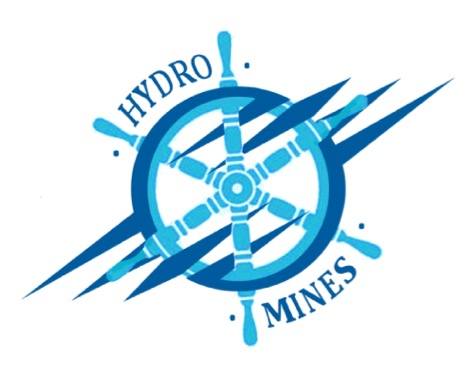
\includegraphics[width=0.7\textwidth]{images/logohydrocontest.jpg}}

\begin{document}

\maketitle

\tableofcontents

\part{Les bateaux}

\chapter{Billy}

\chapter{Billy the Kid}

\chapter{Bateau lourd 2018}
Pour le bateau lourd, nous sommes partis sur un catamaran car le problème de stabilité de la coque ne se posait pas. De plus, on devait à l'époque justifier notre partenariat avec le magazine Multicoque (ce partenariat n'a pas été renouvelé en 2018). Nous sommes donc partis sur une structure en bois qui serait stratifiée.

\section{Conception}
Nous avons regardé différentes coques de catamarans afin de nous familiariser avec leur forme. Nous avons aussi voulu faire une étrave perce-vague.

\subsection{Étrave perce-vaque}
Pour dessiner la forme de l'étrave, nous avons regardé un dessin d'étrave déjà existante. Nous avons ensuite repris l'angle de l'étrave par rapport  l'horizontale.

\subsection{PolyCAD}
Le bateau a conçu à l'aide du logiciel PolyCAD (libre de droit). Nous avons avons voulu faire de l'optimisation de forme de la coque à l'aide de Michlet. Cependant, nous avons du faire face à un grand manque de temps. La forme de la coque a donc été réalisé à l'oeil. Nous avons tout de même minimiser la courbure de la coque. PolyCAD permet en effet d'afficher la courbure des arcs dessinés. Nous avons donc ensuite modifiés les arcs en conséquence.

Un autre facteur très important lors de la conception a été la flottaison du bateau. Nous avions prévu une marge de 12 cm de coque par rapport au niveau de l'eau. En effet, le système de vague créé par le bateau peut être plus grand que le niveau moyen de l'eau. Il a donc fallu modifier les dimensions de la coque pour respecter ces critères. Nous avons privilégié une coque longue et large plutôt que haute. Une coque longue permet d'augmenter la vitesse de coque ($V = \sqrt{L}*2.43$) et une coque large permet d'avoir une plus grande "surface portante".

Nous avons extrait la forme des couples à partir de la forme de la coque: une simple projection sur un plan avec PolyCAD. Les couples ont été espacé régulièrement sauf à l'avant et à l'arrière de la coque, là où la courbure de la coque est la plus grande et où le risque de chocs est le plus grand.

\section{Fabrication}

\subsection{Couples}
Pour faire les couples, nous avons pris des planches d'Oukoumé nautique de de 21 mm. Nous voulions les découper à l'aide de la découpe laser. Cependant, la planche était trop épaisse. Nous aurions du prendre 2 planches plus fines, les mettre en forme à l'aide de la découpeuse laser et les coller ensembles. A défaut de pouvoir cela, nous avons utiliser un vidéo projecteur pour projeter la forme des couples sur le bois. A posteriori, nous aurions tout de même dû utilisé la découpeuse laser pour dessiner les formes à découper sur le bois. Le bois a ensuite été découpé à la scie sauteuse.

Des trous ont été prévus pour faire passer des tasseaux. Ces trous ont été fait en 2 étapes: on a fait 4 trous plus petits qu'on a ensuite enfoncé pour faire un trou plus grand. Ensuite, le trou a été limé pour faire un carré qui laisserait passé tout juste le tasseau.

Les bords des couples ont été poncés afin que ceux-ci fassent un angle. Le clouage des lattes après serait plus simple par la suite.

Les tasseaux ont finalement été insérés dans les couples et les couples ont été positionnés correctement. De la colle à bois a été injectée dans les interstices entre les couples et les tasseaux afin de rigidifier le tout.

\subsection{Lattes}
Nous avons acheté une agrafeuse afin de pouvoir clouer les lattes plus rapidement sur les couples. Le bois choisit pour les lattes est le samba pour sa souplesse et sa légèreté. Nous l'avons acheté chez Weymuller.

Les lattes n'étaient pas assez longues pour faire toute la coque. Nous avons dû les aligner. Nous pensions que faire varier la jonction entre 2 lattes à chaque ligne augmenterait la résistance du montage mais c'est le contraire. Par ailleurs, le fait de monter les lattes ainsi a fait que les lattes n'avaient pas la même courbure une fois sur deux. Nous n'avons pas pu corriger ce défaut lors de la phase de ponçage et de stratification. 

Les lattes ont ensuite été poncées afin que la surface de la coque puissent être stratifiées plus facilement. Cela permet en effet d'éviter de faire des bulles.

\subsection{Stratification de la coque}

\subsection{Les safrans}

\subsection{Les traverses}

\part{Calculs Hydrodynamiques}
Un bon point de départ pour l'Hydrondynamique navale est ce site web qui résume bien tout ce qu'il y a à savoir: \url{https://www.usna.edu/NAOE/academics/en400.php}

Au cours des années, de nombreux logiciels ont été utilisés pour faire des simulations. Voici un récapitulatif de ce qui a été fait.

\chapter{Comment calculer et optimiser la traînée?}

Rédigé par Jean-Baptiste Arber (Hydrocontest 2016-2017 et 2017-2018)

\chapter{Calcul numérique approché de la traînée pour les bateaux fins}

Rédigé par Jean-Baptiste Arber (Hydrocontest 2016-2017 et 2017-2018)

\chapter{Logiciel d'Elie Hachem}

Rédigé par Ulysse Réglage (Hydrocontest 2017)

\textit{NB : Cette note est pour le moment incomplète, mais elle regroupe tout ce que Ulysse Réglade a appris d'Elie Hachem !}

Bon, d’abord il faut se connecter en VPN aux serveurs de Sophia :

\begin{itemize}
\item Lancer Internet Explorer !!! Pas Edge, pas FireFox, non ! Il faut absolument Internet Explorer, aucun autre navigateur ne fonctionnera.
\item Rendez-vous à cette adresse : \url{https://vpn.sophia.mines-paristech.fr/}
\begin{description}
\item[ID:] eleves.mines
\item[Mot de passe:]Hotel..2012
\end{description}
\item Une fois connecté, dites oui à l’installation de ActiveX.
\item Puis, en bas de la page, cliquez sur le serveur Indianola.
\item Normalement, le bureau tout moche de Windows 98 doit apparaitre.
\end{itemize}

Vous être dans la place, vous voulez maintenant faire des simulations, il faut générer les maillages :

\begin{itemize}
\item Tout d’abord, il faut générer des .stl avec un maillage propre, c’est-à-dire régulier, ce que Mr Hachem ne m’a pas encore expliqué comment faire.
\item Puis, il faut générer un maillage volumique pour l’eau et le bateau, en .t, ce que Mr Hachem ne m’a pas non plus expliqué…
\item A la suite de ces 2 étapes, on obtient deux fichiers :
\begin{description}
\item[Domaine.t](le maillage de l’eau).
\item[Object.t ](le maillage du bateau).
\end{description}
\end{itemize}

On va supposer que l’on a ces fichiers pour la suite… Maintenant, il faut lancer les simulations :

\begin{itemize}
\item Le serveur de calcul est le eleves.mines ( Z: ), C’est un 20 cœurs, il apparaît à gauche dans l’explorateur de fichiers.
\item Rendez-vous dans Z:Flow/, vous devez voir des fichiers dont le nom commence par V. Il s’agit des dossiers de simulation. V pour vitesse, la convention et de les nommer par vitesse de simulation (ex : V4 pour 4m/s).
\item Supposons que l’on souhaite faire une simulation pour un écoulement à 4m/s. Prenez l’un des fichiers existant, et copiez-le. Donnez-lui ensuite le bon nom.
\item Allez dans Z:Flow/V4/ et remplacez les fichiers Domaine.t et Object.t.
\item Ouvrez ensuite le fichier Z:Flow/V4/Job/ihm.mtc dans un éditeur de texte, ce sont les paramètres de la simulation :
\begin{description}
\item[PasDeTemps]précision temporelle de la simulation en secondes, 0.1 c’est bien !
\item[TempsFin]durée de la simulation, 500 est une bonne valeur pour Elli.
\item[VIn]est la vitesse de l’écoulement en m/s.
\end{description}
\item Pensez bien à modifier VIn et à enregistrer les modifications
\end{itemize}

\begin{figure}[h]
	\begin{center}	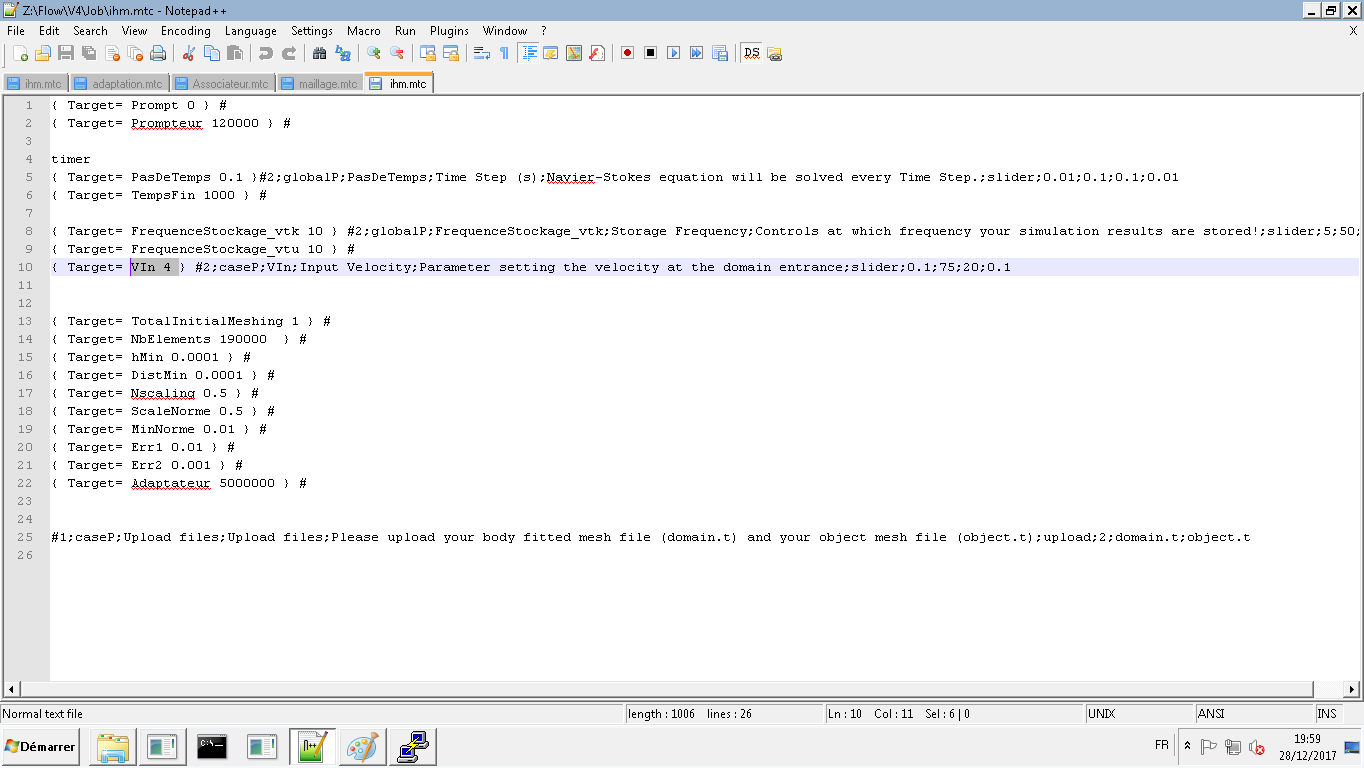
\includegraphics[width=0.5\textwidth]{images/CFD1.png}
	\end{center}
\end{figure}

\begin{itemize}
\item Enfin, allez dans Z:Flow/V4/Job/result/ et supprimez bien tous les fichiers en .vtu.
\end{itemize}

Maintenant, il faut lancer la simulation :

\begin{itemize}
\item Allez dans démarrer, et tapez putty, puis entre.
\end{itemize}

\begin{figure}[h]
	\begin{center}	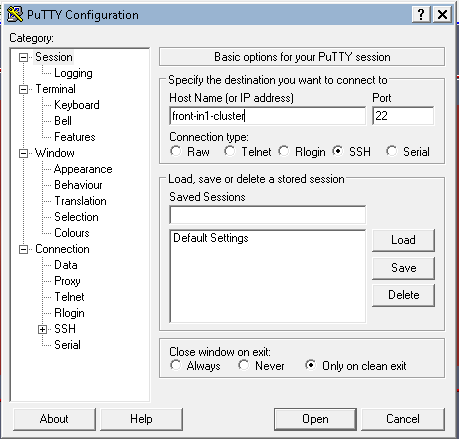
\includegraphics[width=0.6\textwidth]{images/CFD2.png}
	\end{center}
\end{figure}

\begin{itemize}
\item Pour vous connectez au cluster, rentrez front-in1-cluster dans Host Name. Puis Open, et rentrez le nom d’utilisateur et le mot de passe donnés plus haut, c’est les mêmes.
\item La console s’affiche 
\end{itemize}

\begin{figure}[h]
	\begin{center}	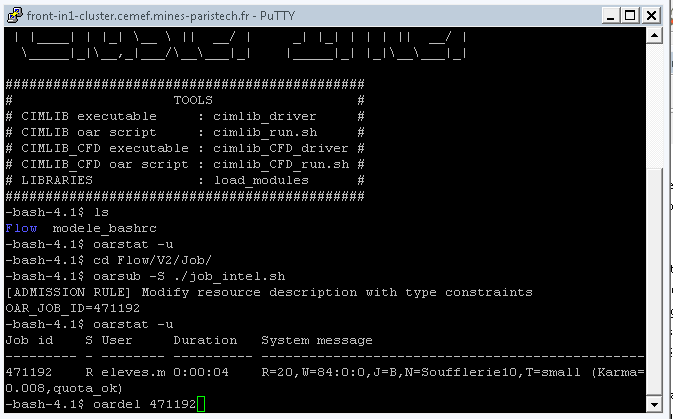
\includegraphics[width=0.7\textwidth]{images/CFD3.png}
	\end{center}
\end{figure}

\begin{itemize}
\item Vous aurez besoin de 3 commandes :
\begin{description}
\item[oarstat –u ](Pour afficher les calculs en cours)
\item[oardel 470643 ](Pour tuer en calcul, le numéro étant l’id du calcul affiché par la commande précédente)
\item[oarsub -S ./job\_intel.sh ](La commande pour lancer un calcule, à lancer dans le fichier Job)
\end{description}
\item Les résultats de simulation apparaissent dans le dossier Z:Flow/V4/Job/result/, ce sont les fichiers .vtu.
\end{itemize}

Pour visualiser les résultats :

\begin{itemize}
\item Lancer le logiciel paraview depuis le menu démarrer.
\item Ouvrez le vtu que vous voulez.
\item Un gros pavez apparaît, c’est l’eau, zoomez à l’intérieur pour trouver le bateau.
\item Pour afficher le champ dans vitesses et des pressions, ajoutez une nouvelle slice (en haut à gauche), et cochez pression ou vitesse dans le menu déroulant en haut à gauche.
\item Utilisez la souris pour bouger la coupe et tourner la vue.
\end{itemize}

\begin{figure}[h]
	\begin{center}	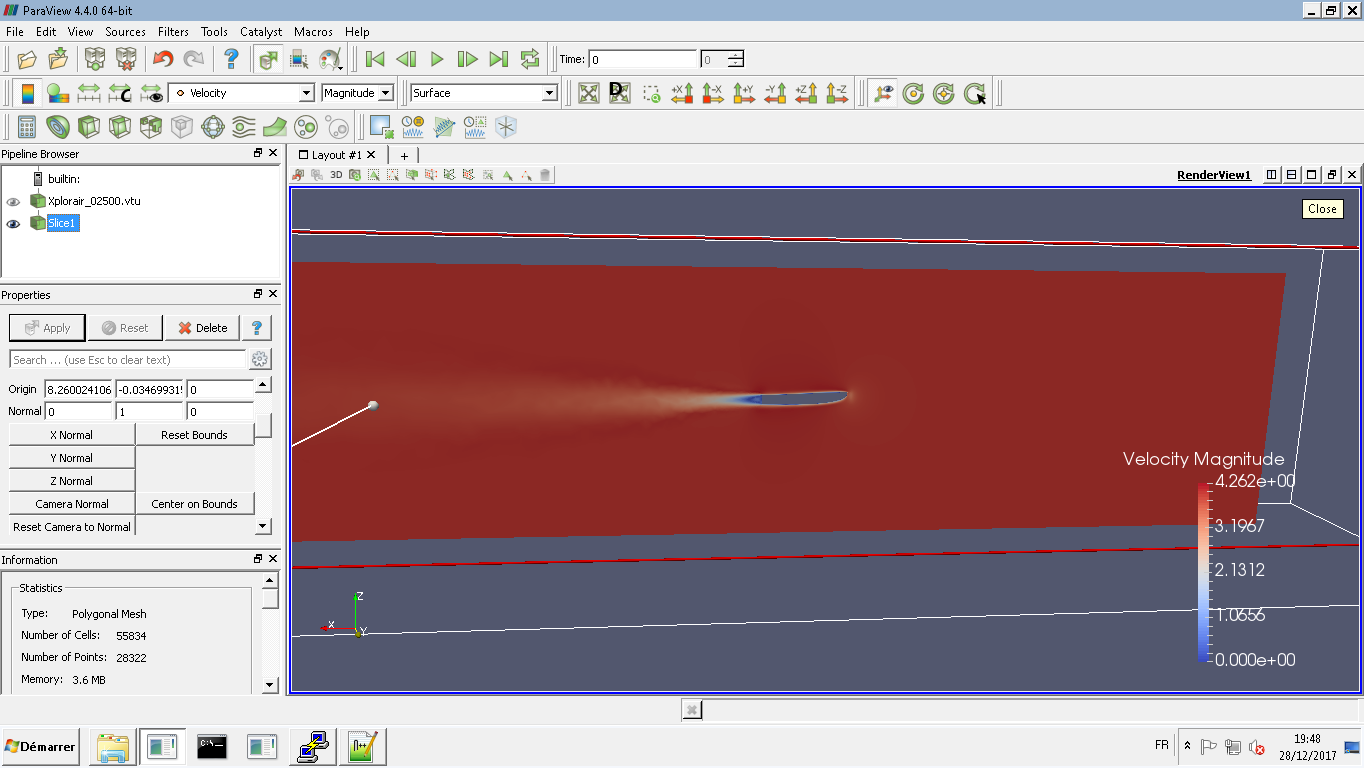
\includegraphics[width=0.7\textwidth]{images/CFD4.png}
	\end{center}
\end{figure}

\begin{itemize}
\item Pour le moment, c’est du monophasique, le bateau est donc un sous-marin.
\item Mr Hachem n’a pas fait la routine pour intégrer le champ des pressions, on a donc pas la résistance à l’avancement.
\item Je peux interpoler le champs des pressions sur la coque du bateau, mais je suis en déplacement, et mes notes sont à Toulouse.
\end{itemize}

\chapter{Logiciel: Fine Marine}

\part{CAO}

\chapter{PolyCAD}

\part{Les outils à disposition}

\chapter{Les outils de la menuiserie}
La menuiserie possède pas mal d'équipement à la disposition des élèves. Il n'y a pas trop de restrictions sur leur utilisation à condition de tout ranger après à moins de vouloir faire face à Jacky, le responsable de la menuiserie. Il ne faut d'ailleurs pas hésiter à lui demander conseil si besoin est, il est toujours prêt à aider les étudiants dans leurs projets.

Le responsable des outils avancés de la menuiserie est Henri Proudhon. C'est celui qu'il faut contacter si jamais vous souhaitez apprendre à utiliser l'une des machines.

\section{L'imprimante 3D}
L'école possède pour l'instant 3 imprimantes 3D. Vous n'utiliserez très probablement jamais la plus ancienne. Les 2 que seront utiles sont:
\begin{description}
\item[l'Ultimaker 2+:]C'est celle qui peut imprimer le plus grand volume: 223 x 223 x 305 mm
\item[l'Ultimaker 3:]La version la plus récente. Elle permet d'imprimer un volume plus faible que l'Ultimaker 2+ (215 x 215 x 200 mm) mais elle possède 2 têtes d'impressions ce qui lui permet de faire des impressions avec 2 matériaux différents.
\end{description}

\begin{figure}[h]
	\begin{center}
		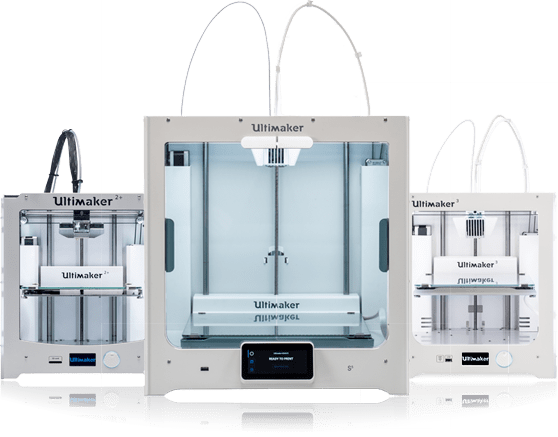
\includegraphics[scale=0.6]{images/ultimaker.png}
		\caption{Les imprimantes 3D Ultimaker}
	\end{center}
\end{figure}

\subsection{Le logiciel: Cura}
Cura est le logiciel qui permet de créer le fichier qui sera utilisé par les Ultimakers. On peut définir les paramètres d'impressions et le positionnement des objets à imprimer dans l'imprimante 3D. 

Attention, l'Ultimaker 3 ne fonctionne pas pour l'instant avec la version 3.3.1 de Cura. Il faut utiliser la version 3.2.1.

\begin{figure}[h]
	\begin{center}
		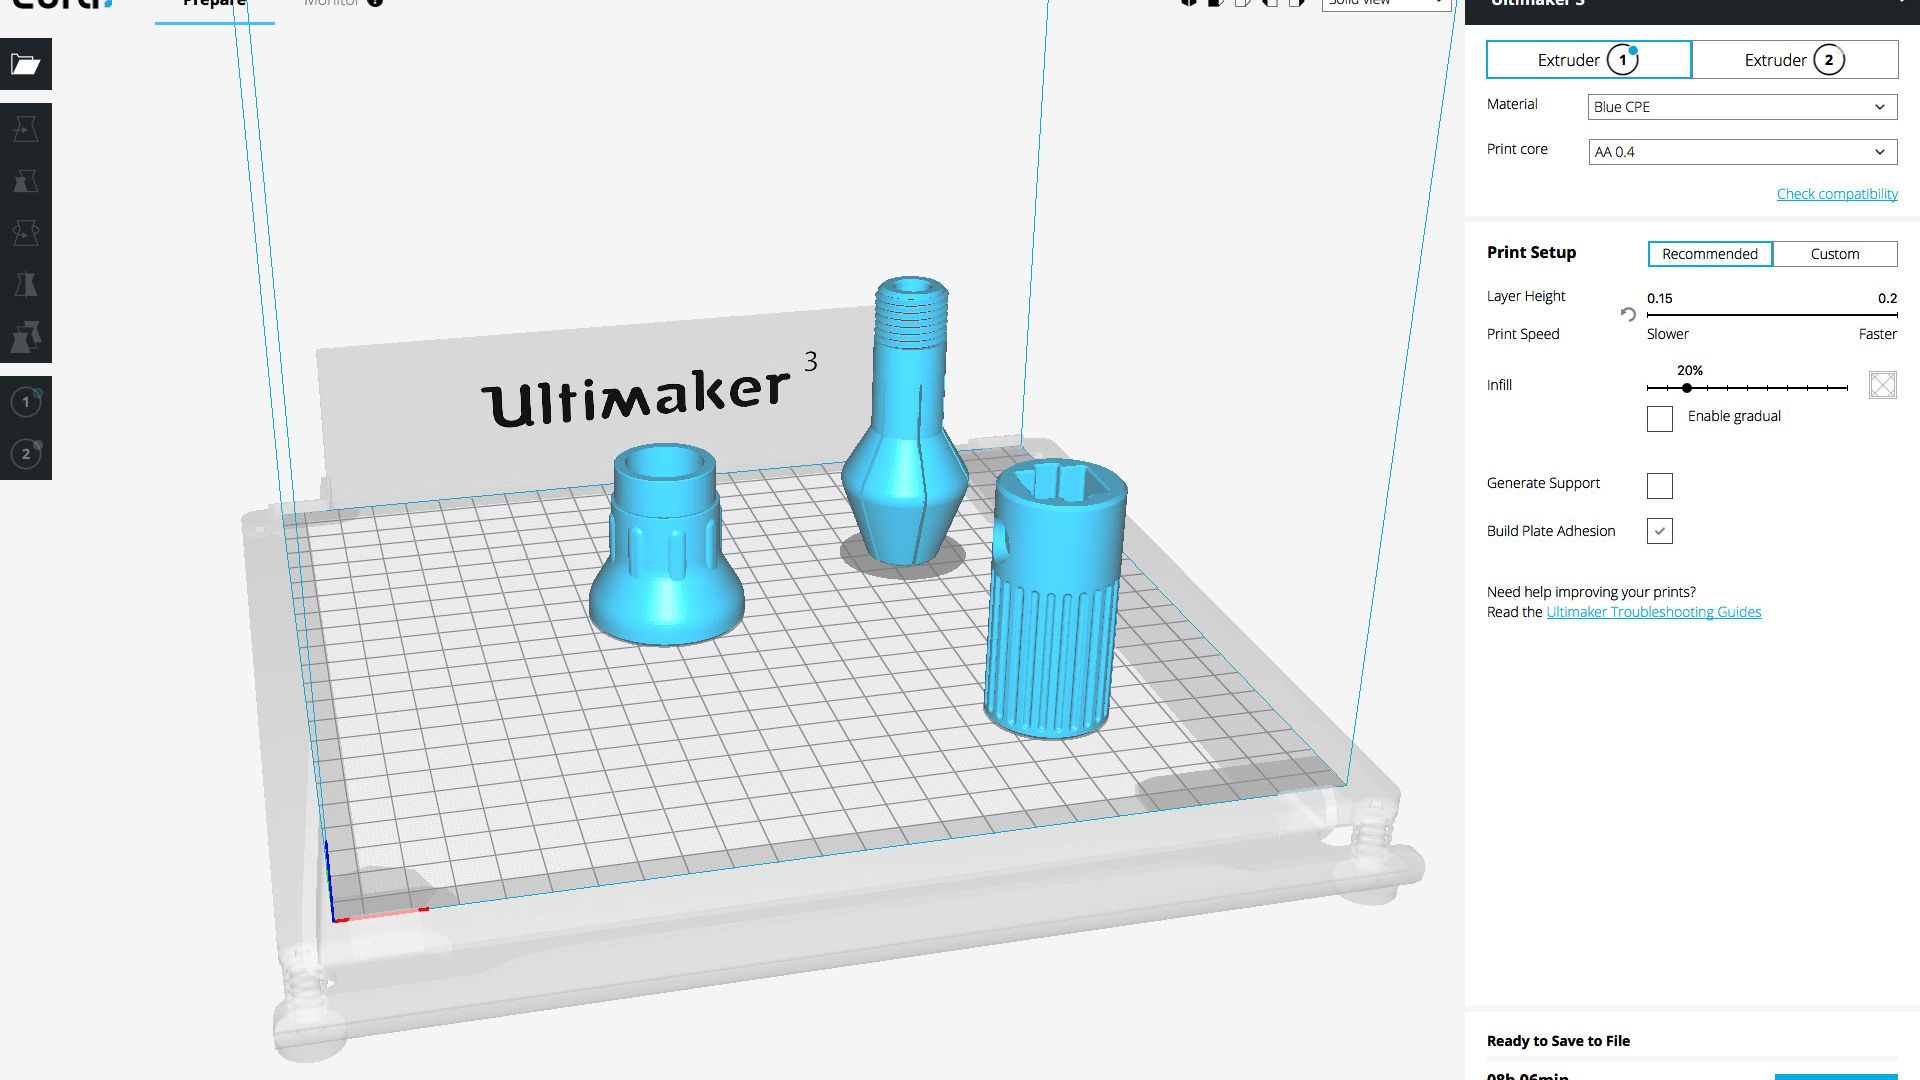
\includegraphics[width=0.5\textwidth]{images/cura.jpg}
		\caption{Cura}
	\end{center}
\end{figure}

\subsection{Utilisation}
Avant de lancer l'impression, il faut passer un coup de spray dur le plateau d'impression. Cela évite d'avoir des problèmes quand on décollera l'impression à la fin.

Le menu est très intuitif et bien expliqué. Le changement des bobines est aussi très simple et bien expliqué sur le site web d'Ultimaker.

\section{La découpeuse laser}
La découpeuse laser est plus complexe à utiliser que l'imprimante 3D. Il vaut mieux que Henri Proudhon vous montre précisément comment l'utiliser. Il faut en effet choisir des paramètres spécifiques à chaque matériaux. Des paramètres sont déjà définis dans la machine pour certains matériaux mais il faudra très certainement mettre cela à jour avec de nouveaux matières premières. Ensuite, il faut calibrer la distance du laser au matériau à découper afin que cela corresponde à la distance focale. C'est d'ailleurs pour cela qu'il est impossible de couper des matériaux d'une trop grande épaisseur (21mm ne passent pas je crois). On peut contourner ce problème en découpant plusieurs fois le même motif et en les empilant par contre.

La découpeuse laser accepte seulement des matériaux de 40 x 80 cm (à revérifier). Cependant, la découpeuse laser s'ouvre sur un côté. Cela permet d'insérer dedans de pièces qui font plus de 40 cm de largeur.

Certaines matières plastiques ne peuvent être découpées par la découpeuse laser car ils produisent des fumées toxiques lorsqu'ils brûlent. Il faut alors utiliser une fraiseuse CNC (qui est en réparation).

\begin{figure}[h]
	\begin{center}
		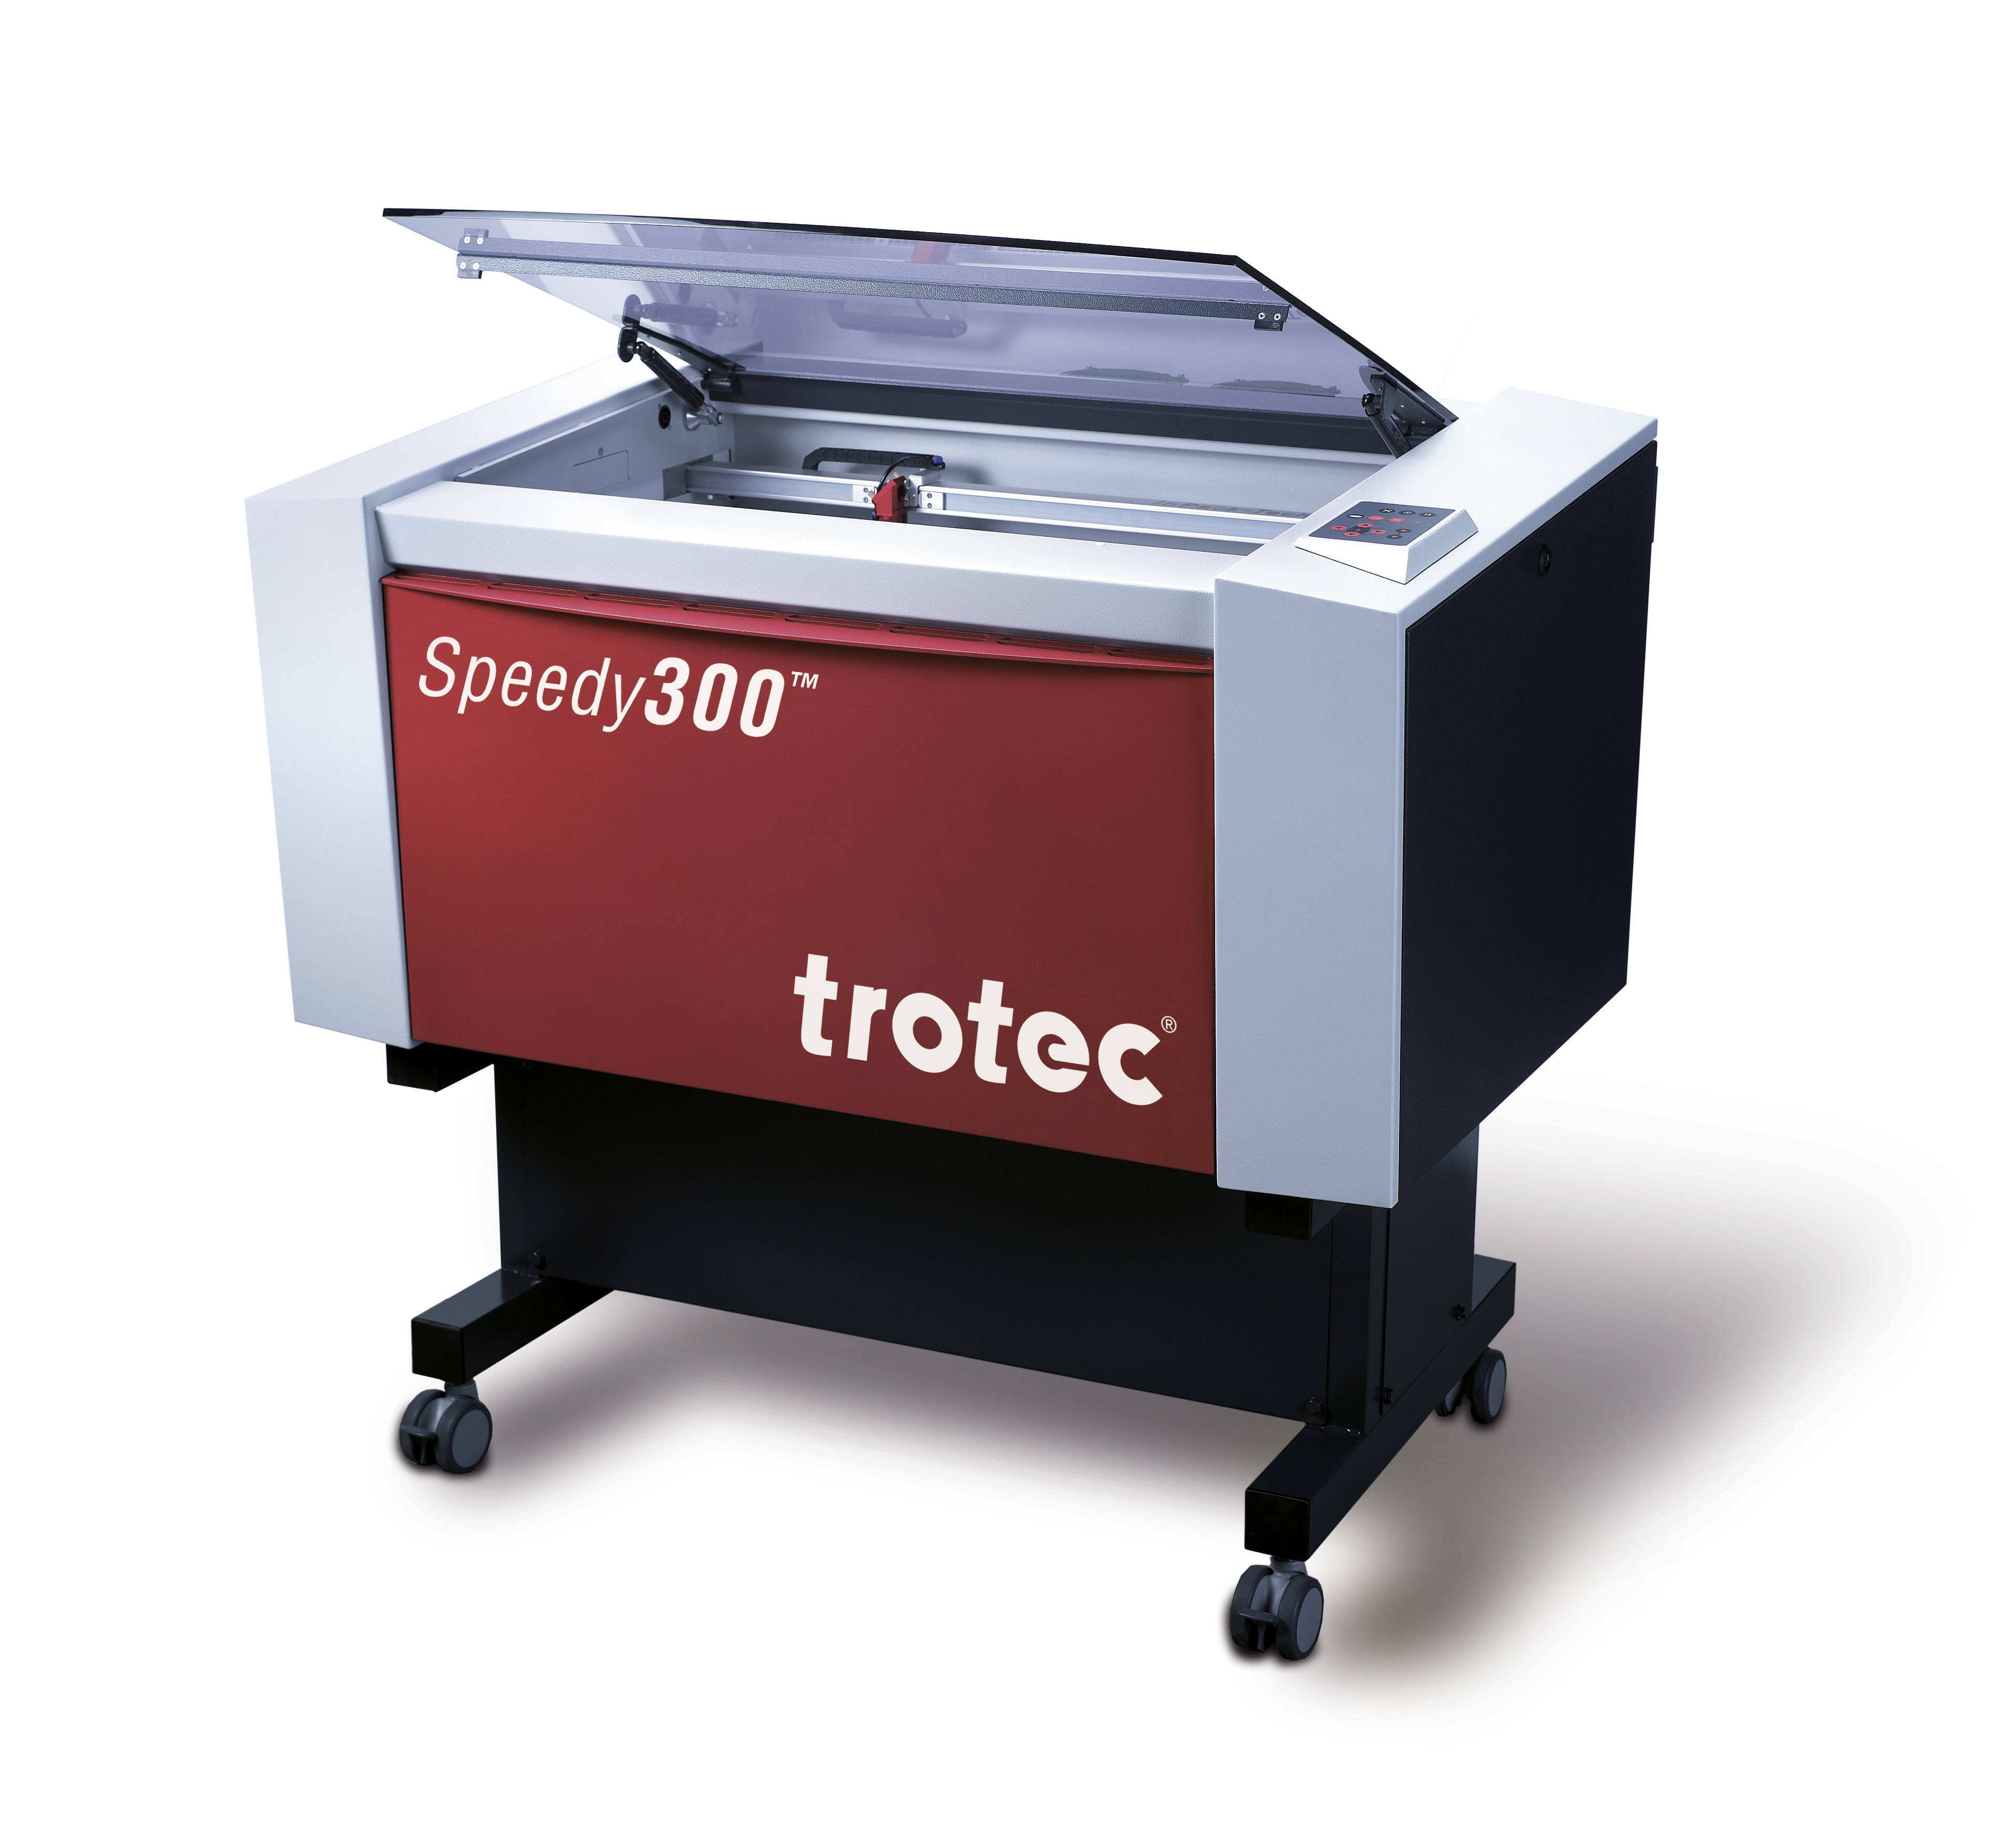
\includegraphics[width=0.5\textwidth]{images/decoupeuse_laser.jpg}
		\caption{Découpeuse laser}
	\end{center}
\end{figure}

\subsection{Le logiciel: Inkscape}
Inkscape est un logiciel de traitement graphique. C'est celui qui produit les fichiers acceptés par la découpeuse laser. Si vous souhaitez découper quelque chose, il faut que votre dessin soit importer sous Inkscape, mis à l'échelle (attention aux unités utilisés) puis il faut que le trait soit en rouge afin qu'il soit reconnu par la découpeuse laser.

\begin{figure}[h]
	\begin{center}
		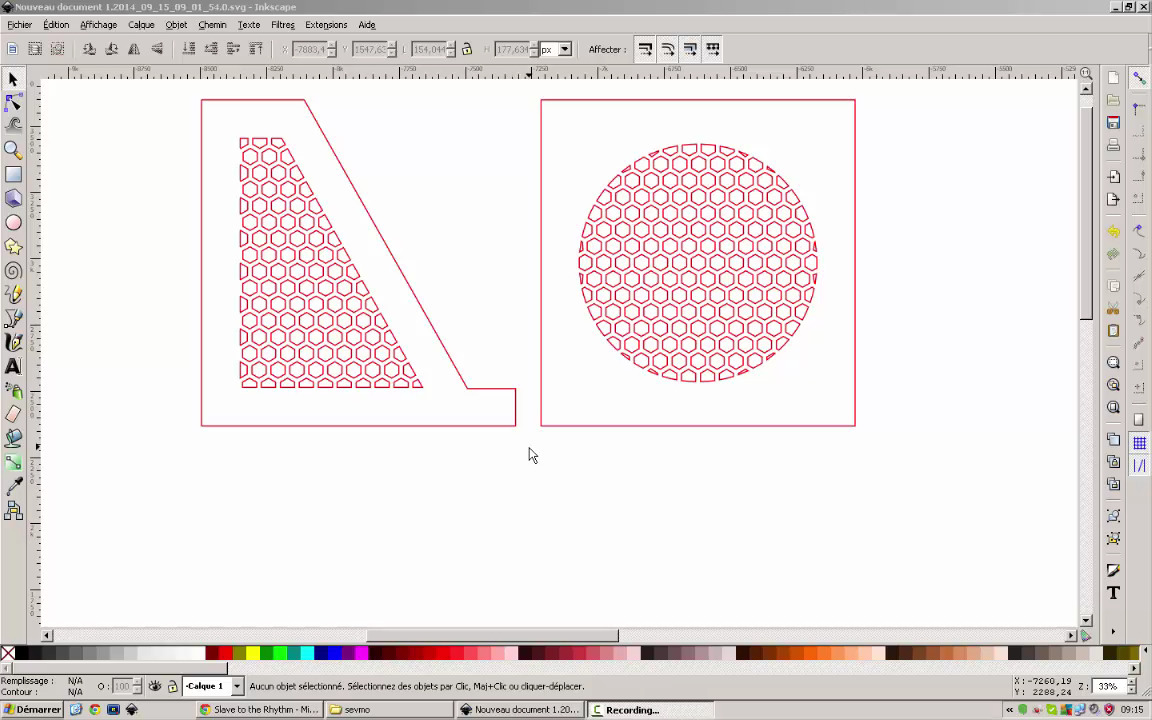
\includegraphics[width=0.5\textwidth]{images/inkscape.jpg}
		\caption{Inkscape}
	\end{center}
\end{figure}

\chapter{Le matériel de stratification}

\part{Le matériel}

\chapter{Objectif de cette partie}

Au cours des deux campagnes hydrocontest auxquelles j'ai participé,
j'ai notamment été en charge de trouver et commander tous les composants
servant à fabriquer le système électronique du bateau au sens large,
c'est à dire :
\begin{enumerate}
\item les composants pûrement électroniques, de faible puissance (micro-contrôleur,
capteurs, modules radio ...etc)
\item les composants électriques, dont certains doivent gérer des puissances
importantes (fusibles, porte-fusibles, interrupteurs ...etc)
\item le matériel servant à relier tous ces composants entre eux pour réaliser
les circuits
\item les boîtiers étanches servant à protéger les circuits des chocs, de
l'eau...etc
\item le circuit de refroidissement, servant à refroidir certains composants,
ou l'air de certains boîtiers
\item le matériel permettant de réaliser des connexions étanches entre les
boîtiers, ou entre un boîtier et un composant situé à l'extérieur,
que ce soit une connexion électrique (par exemple entre la batterie
et le variateur s'ils sont dans des boîtiers séparés), ou hydraulique
(circuit de refroidissement). Ces connexions doivent aussi être pensées
pour être facilement défaites et refaites, lors de la maintenance
du bateau.
\end{enumerate}
Rappelons que le système électronique n'est pas forcément intégralement
situé sur le bateau, il peut y en avoir une partie à quai avec le
pilote par exemple.

Pourquoi faire un REX là-dessus ? Tout simplement parce que commander
tout cela est un peu plus compliqué que d'aller acheter une planche
de bois chez Leroy Merlin, et ceci pour deux principales raisons : 
\begin{enumerate}
\item On parle ici de produits spécialisés, et il faut donc avoir une certaine
expérience ou avoir fait beaucoup de recherches sur internet (c'est
mon cas, ça prend un temps fou, d'où l'intérêt de ce REX) pour trouver
le produit adapté et comment il s'appelle : savez-vous par exemple
que le produit idéal pour faire passer des cables à travers un boîtier
de manière étanche s'appelle un presse-étoupe (cable gland en anglais)
? Si vous ne le savez pas, vous allez galérer pour le trouver la première
fois parce que googler ''comment faire passer des cables de manière
étanche à travers un boîtier'' ne donne pas immédiatement le bon
résultat.
\item Il faut savoir où trouver ces produits (oubliez Leroy Merlin, amazon,
ebay et même RS pour certains d'entre eux) et si possible savoir où
les trouver au bon prix.
\end{enumerate}
Il est donc essentiel de se passer les infos d'année en année pour
ne pas avoir à refaire ce long travail de recherche. Par ailleurs,
acheter les bons composants à temps dans les bonnes quantités est
un travail crucial :
\begin{enumerate}
\item Ne pas avoir les composants à temps implique soit bloquer le projet,
soit trouver une solution alternative, qui le plus souvent est de
piètre qualité et fait perdre beaucoup de temps. Le pire est quand
cela arrive lors de la compétition, et prévoir quoi apporter sur place
est donc une question vitale.
\item Ne pas bien gérer les approvisionnement implique des aller-retours
supplémentaires, parfois infructueux, dans des magasins, et donc une
perte de temps considérable.
\end{enumerate}
Pour résumer, ne pas anticiper suffisament la conception du système
électronique (qui peut-être assez complexe mine de rien avec toutes
les contraintes d'étanchéité, de praticité, de sécurité ...etc) et
la commande des composants résultera forcément en un travail de qualité
moyenne, des crises de nerfs, et dans le pire des cas à un bateau
qui ne fonctionne pas le jour j.

Il est souvent tentant de réfléchir à un système électronique sophistiqué
et performant, mais avant cela il faut déjà être capable de réaliser
un système simple mais robuste (circuits de qualité, bien protégés,
bien étanches ...etc). Prévoir des choses compliquées sans maîtriser
la base est la recette d'un échec assuré !

Maintenant que je vous ai convaincu de l'importance de ce document
(du moins j'espère), je vais aborder plein de composants un peu en
vrac, en les regroupant néanmoins par catégories. Ensuite, je ferai
un bilan des différents fournisseurs que j'évoque dans ce document.

Notez que je n'écris pas de REX complet sur la conception du système
électronique / électrique, parce que la plupart des problématiques
tiennent de la bonne connaissance du réglement et du bon sens (par
exemple bien dimensionner les conducteurs en fonction de l'intensité
du courant, prévoir assez de place dans les boîtiers...etc). N'hésitez
pas à me contacter cependant si vous avez des questions.

Une dernière remarque : je soulignerai souvent la nécessité d'avoir
sous la main certains composants, n'allez pas les acheter avant de
vérifier ce qu'hydromines possède déjà comme matériel (nous avons
déjà accumulé pas mal de composants et d'outils). Je mentionne dans
ce document l'achat de composants que nous possédons déjà car ce guide
se doit d'être le plus général possible.

\chapter{Composants pûrement électroniques}

\section{Système de contrôle}
Afin de pouvoir commander le bateau à distance, on a décidé d'utiliser comme la plupart des équipes une radiocommande et un récepteur de modélisme.

\subsection{Radiocommande}
La radiocommande choisi est la Taranis X9D. C'est la meilleur en terme de qualité-prix. Elle est totalement programmable (à entendre dans le sens de paramétrable) et la communauté autour est très grande. Si jamais, il y a un problème, il suffit juste de chercher sur les forums.

\begin{figure}[h]
	\begin{center}
		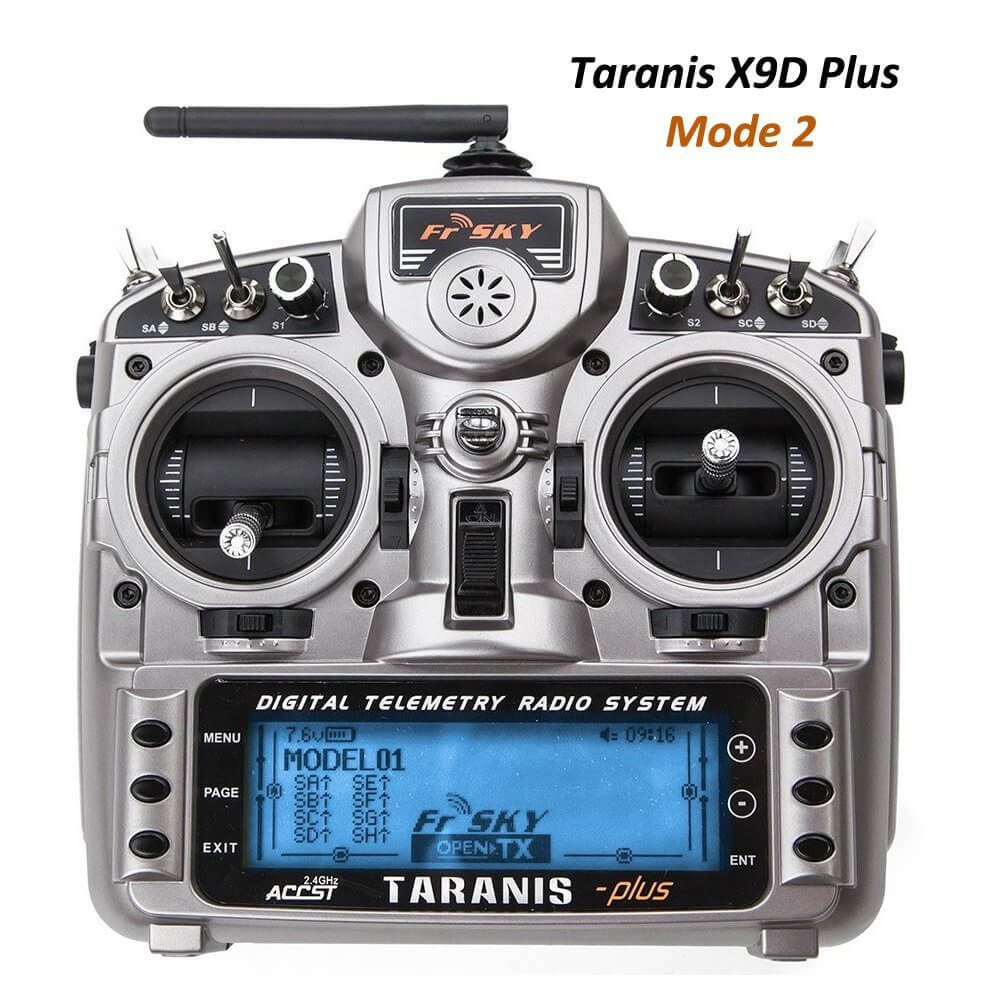
\includegraphics[width=0.5\textwidth]{images/taranis.jpg}
		\caption{Taranis X9D}
	\end{center}
\end{figure}

Les radiocommandes existent sous plusieurs modes. Ces modes définissent à quelle manette vont être attribuées quelles fonctions. Il faut savoir que les manettes ne sont pas identiques (il peut y avoir un ressort qui les recentrent ou non).

\begin{figure}[h]
	\begin{center}
		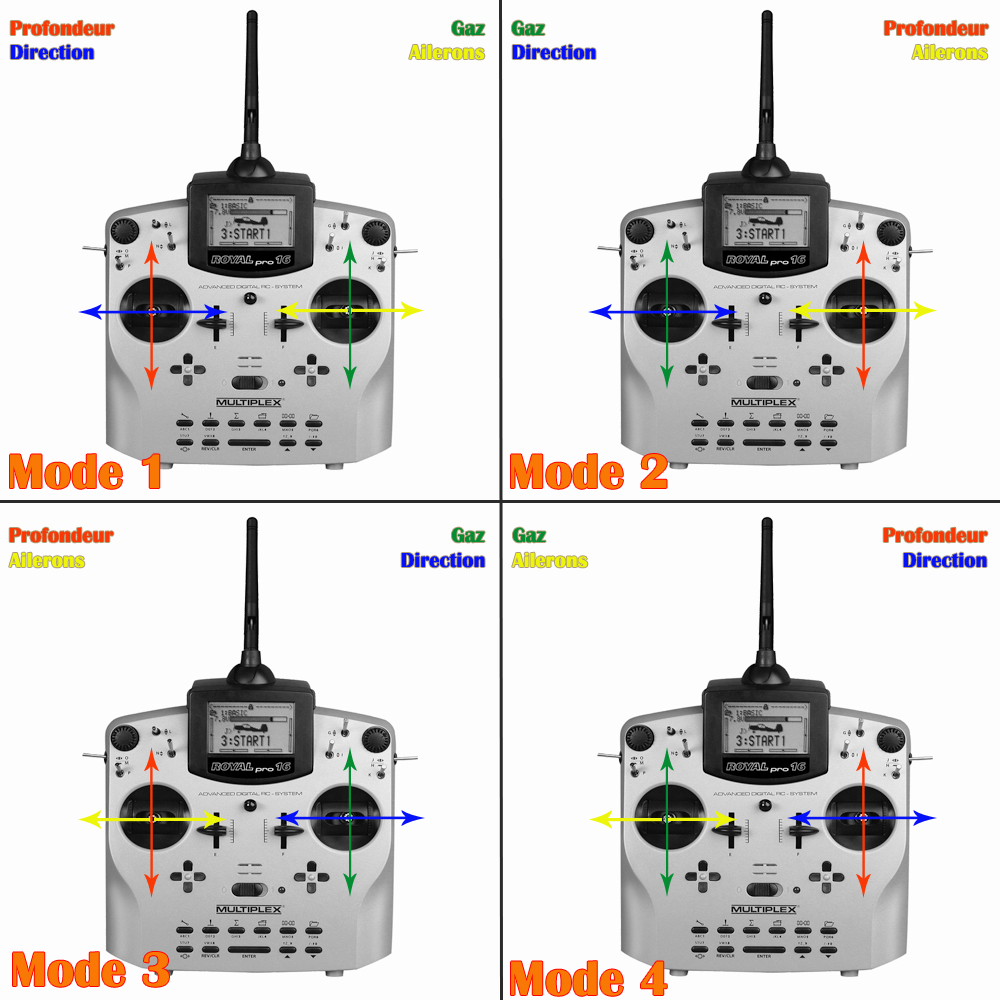
\includegraphics[width=0.5\textwidth]{images/mode_radiocommande.jpg}
		\caption{Modes de pilotages pour radiocommande}
	\end{center}
\end{figure}

La taranis fonctionne à une fréquence de 2.4GHz (c'est d'ailleurs la même fréquence que le Wifi). Auparavant, les fréquences utilisés étaient le 42MHz et le 58MHz. Cependant, ces fréquences étaient partagés en plusieurs sous-fréquences et on ne pouvait être qu'un seul utilisateur par fréquence. L'avantage du 2.4GHz est que l'antenne est plus petite grâce à la plus faible longueur d'onde et chaque récepteur est "bindé" à une seule radiocommande. Cependant, on perd en porté et en pouvoir pénétrant des ondes.

Ce qu'il est possible de faire avec la Taranis:
\begin{itemize}
\item Paramétrer le signal envoyé au récepteur en fonction des commandes (loi linéaire, exponentielle, choisir les paramètres de la loi,...). C'est notamment utile quand les câbles du moteur brushless triphasé sont mal branchés. La manette des gaz est alors inversés. On peut régler ce problème directement en faisant une loi de commande linéaire avec une pente de -1 pour le moteur.
\item Faire de la télémétrie avec l'équipement approprier. Cependant, on fait la télémétrie totalement à part.
\item Chronométrer les performances avec un chronomètre embarqué
\item Pleins d'autres choses, à voir en fonction des besoins.
\end{itemize}

\subsection{Récepteur}
De nombreux récepteurs radios sont compatibles avec la Taranis. Ce sont ceux du même fournisseur qui ont été choisis: FrSky. On utilise le X4RSB.

\begin{figure}[h]
	\begin{center}
		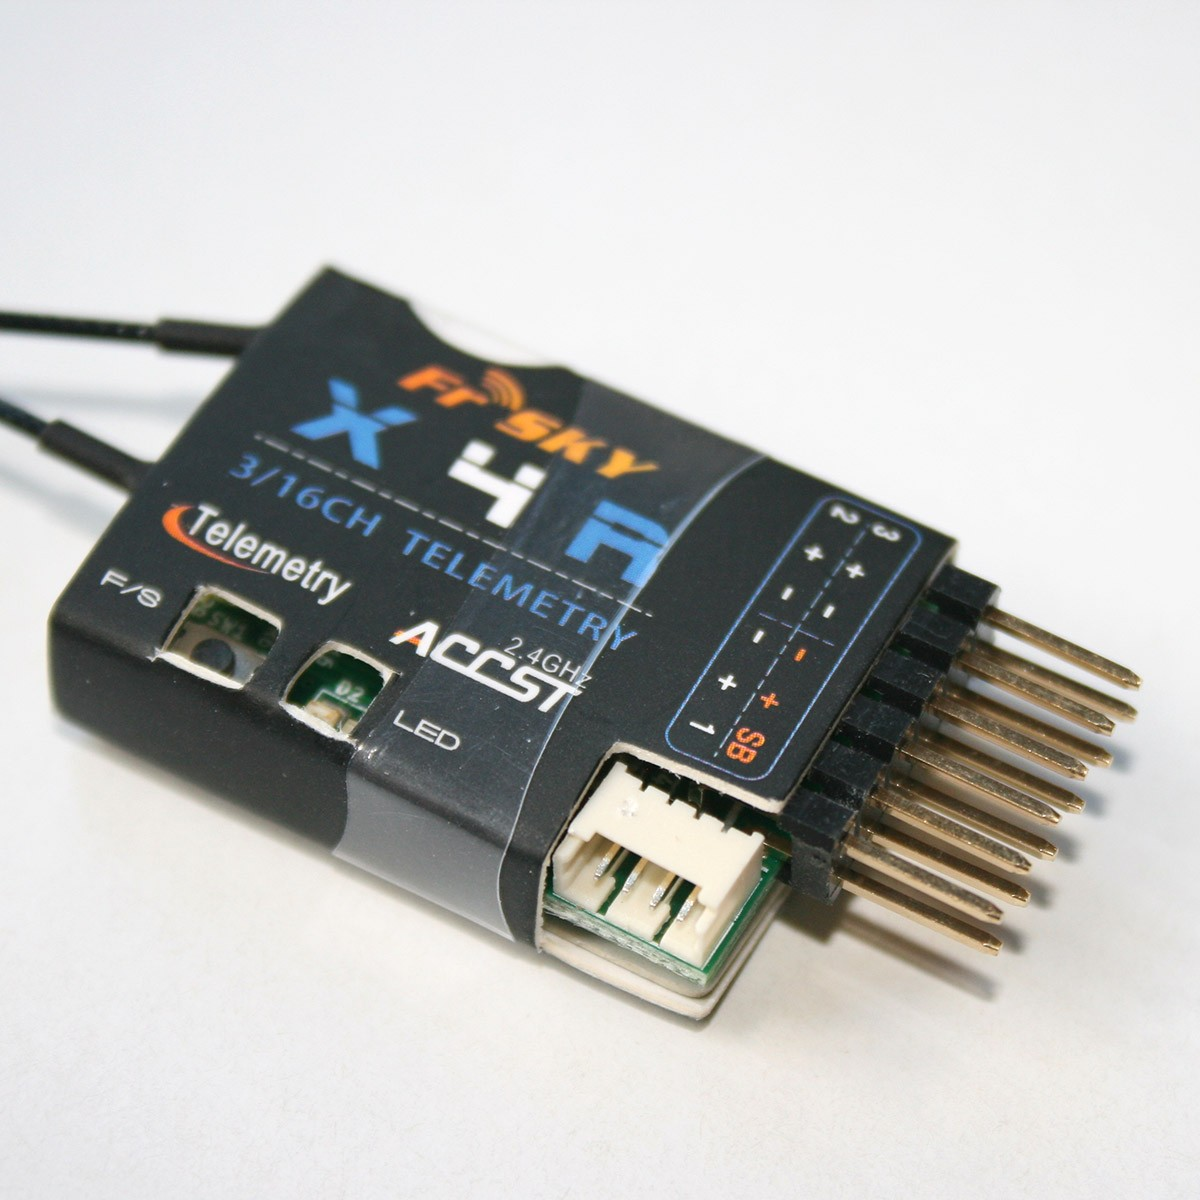
\includegraphics[width=0.5\textwidth]{images/X4RSB.jpg}
		\caption{Récepteur X4RSB de FrSky}
	\end{center}
\end{figure}

C'est le meilleur choix en terme de rapport qualité/prix et il convient parfaitement à nos besoins. De nombreux autres modèles sont disponibles sur leur site.

\subsubsection{Paramétrage du récepteur}
Avant de pouvoir utiliser le récepteur, il faut faire 2 choses: le "binder" avec la radiocommande et paramétrer le mode par défaut c'est-à-dire comment il va se comporter si jamais il perd le signal radio. Les protocoles à suivre sont sur la documentation du récepteur disponible sur internet.

\section{Communication radio}

\begin{figure}[h]
\caption{Un module Xbee (gauche) / Xbee Explorer Regulated (droite)}

\begin{centering}
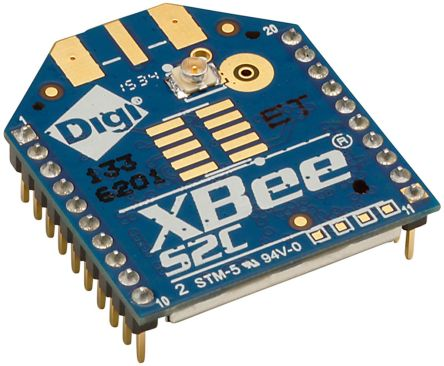
\includegraphics[width=0.5\textwidth]{images/xbee}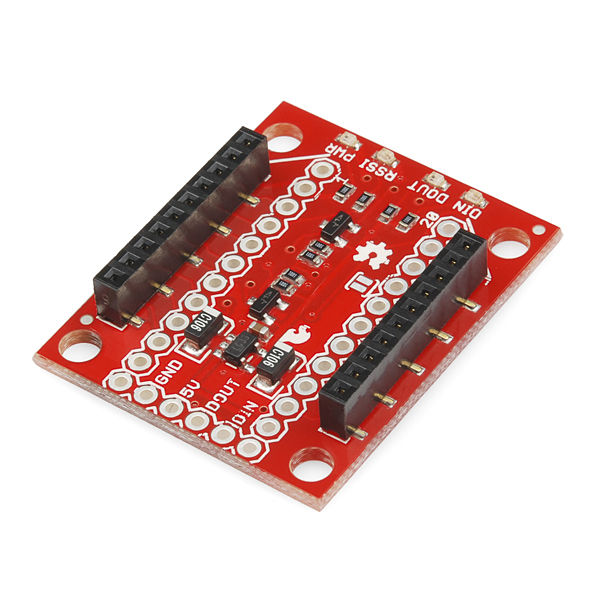
\includegraphics[width=0.5\textwidth]{images/xbee_explorer_regulated.jpg}
\par\end{centering}
\end{figure}

Les modules radio Xbee sont une solution robuste pour transmettre
des données. Ils peuvent être configurés de plein de façons différentes,
et il est ainsi possible de créer des réseaux de communication complexes
avec de nombreux modules, ou bien plus simplement de remplacer une
liaison série cablée par un canal radio entre deux modules. Certains
modules ont une antenne intégrée, certains ont une prise pour antenne
externe. Attention, la portée et le débit de ces modules varient énormément
d'un modèle à l'autre, puisque différents modèles utilisent des technologies
différentes.

Ils se connectent à un ordinateur ou micro-contrôleur par un adaptateur
USB, ou par un adaptateur vers liaison série, comme le XBee Explorer
Regulated.

En cas d'utilisation d'antenne externe, le plus simple est d'opter
pour un Xbee avec connecteur SMA ou RP-SMA. On trouve facilement des
antennes de ce type sur amazon ou chez le fournisseur tme.eu à très
bon prix. Faites attention à prendre une antenne prévue pour la bonne
fréquence, et de gain suffisant.

S'il faut déporter l'antenne, on trouve des cables de rallonge SMA
facilement sur tme.eu dans la catégorie des cables coaxiaux.

\section{Utiliser internet en cas de perte de la liaison radio}

N'oubliez pas que, les bateaux ne s'éloignant jamais trop de la terre
ferme, il y a de bonnes chances pour que le bateau puisse capter le
réseau mobile et se connecter à internet (il faut pour cela qu'il
y ait un micro-ordinateur à bord auquel on connecte une clef 4G par
exemple).

Si c'est le cas, et si le système de pilotage est aussi connecté à
internet, il est possible de mettre en place une liaison de données
à faible latence en utilisant le protocole MQTT (simple à utiliser
avec des librairies faciles à prendre en main dans de nombreux langages
de programmation), qui permet d'atteindre des latences très faibles
en choisissant la QoS (quality of service) la plus faible.

\section{Transmission vidéo analogique}
On trouve facilement le matériel nécessaire pour transmettre de la
vidéo analogique par radio sur le canal 5.8 GHz sur les sites de matériel
de modélisme, puisque c'est la principale méthode employée notamment
en aéromodélisme.

Si cela vous intéresse, vous pouvez vous renseigner plus en profondeur sur ce site: oscarliang.com. Il est très bien fait.

\subsection{Émetteur vidéo VTX}
Modèle choisi: Matek HV VTX

\begin{figure}[h]
	\begin{center}
		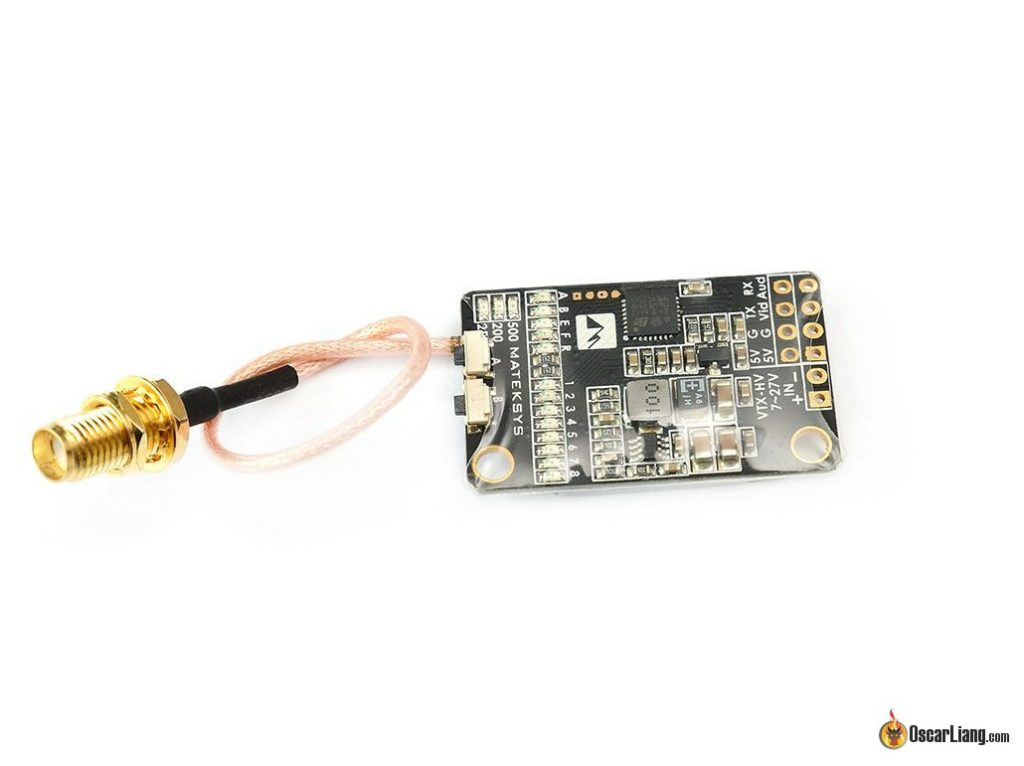
\includegraphics[width=0.5\textwidth]{images/vtx.jpg}
		\caption{Matek HV VTX}
	\end{center}
\end{figure}

\begin{itemize}
\item VTX signifie Video Transmitter.
\item L'émetteur  chauffe très rapidement, il faut donc s'assurer qu'il doit bien refroidi.
\item L'antenne doit TOUJOURS être branchée à l'émetteur vidéo lorsque celui-ci est mis sous tension. En effet, sans l'antenne, l'émetteur vidéo ne peut disperser l'énergie absorbée.
\end{itemize}

\url{https://oscarliang.com/choose-video-transmitter-fpv-mini-quad/}

\subsection{Récepteur vidéo (Écran)}
Modèle choisi: 7 inch 800 x 480 40CH Diversity Receiver Sun Readable FPV Monitor w/DVR Fieldview 777SB

\begin{figure}[h]
	\begin{center}
		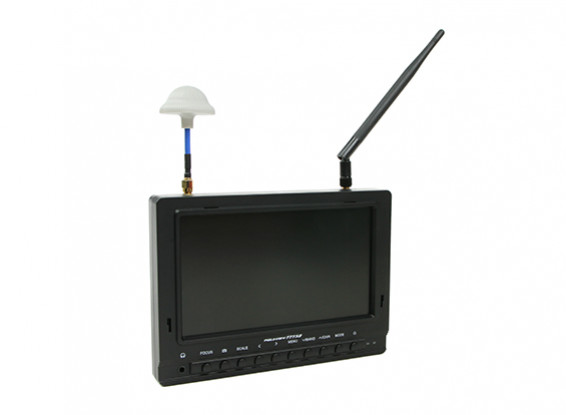
\includegraphics[width=0.5\textwidth]{images/ecran.jpg}
		\caption{Ecran FPV}
	\end{center}
\end{figure}

\begin{itemize}
\item Il faut mettre 2 types d'antennes différentes afin que leur "profil de réception" se complémentent.
\end{itemize}

\subsection{Caméra}
Modèle choisi: Runcam Eagle 2

\begin{figure}[h]
	\begin{center}
		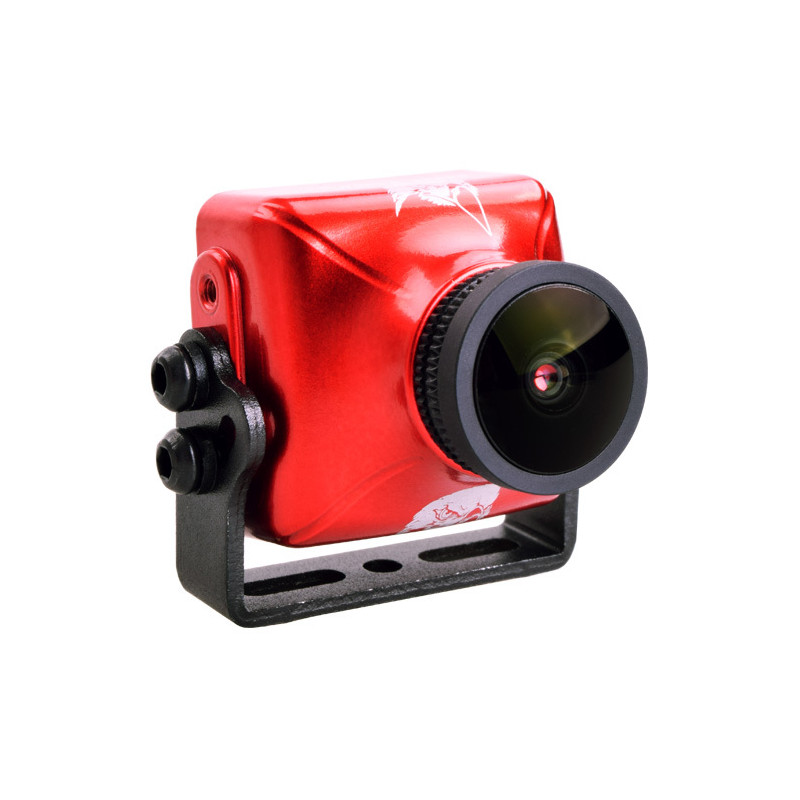
\includegraphics[width=0.5\textwidth]{images/camera.jpg}
		\caption{Runcam Eagle 2}
	\end{center}
\end{figure}

Afin d'obtenir la meilleure retransmission vidéo, il faut jouer sur tout les paramètres vidéos (contraste, luminosité,...).

\url{https://oscarliang.com/fpv-camera-settings/}

Le champ de vue de la caméra dépend de la lentille utilisé.

\url{https://oscarliang.com/fpv-camera-lens/}

\subsection{Les antennes}
Modèle choisi: Aomway 4-lobe Cloverleaf

\begin{figure}[h]
	\begin{center}
		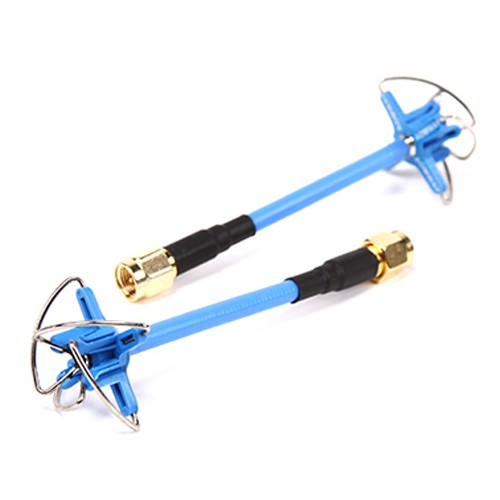
\includegraphics[width=0.5\textwidth]{images/antenne.jpg}
		\caption{Aomway 4-lobe Cloverleaf}
	\end{center}
\end{figure}

\begin{itemize}
\item Les antennes sont très fragiles. C'est leur forme qui assure la bonne transmission du signal. Il ne faut donc pas les tordre.
\item Il existe différents types de connecteurs à différencier.
\end{itemize}

\begin{figure}[h]
	\begin{center}
		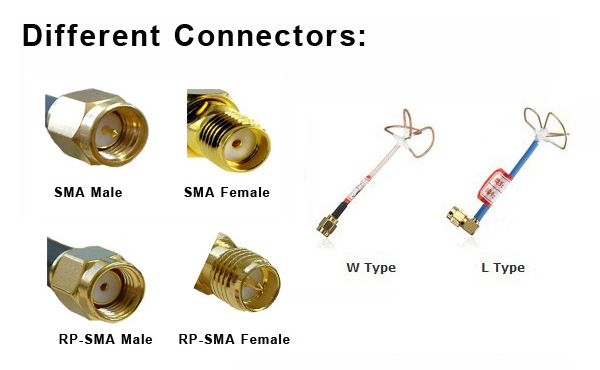
\includegraphics[width=0.5\textwidth]{images/connecteur_antenne.jpg}
		\caption{Les différents types de connecteurs pour les antennes}
	\end{center}
\end{figure}


\url{https://oscarliang.com/best-fpv-antenna/}

\section{Micro-ordinateurs}

\begin{figure}[h]
\caption{Raspberry Pi Zero W}

\centering{}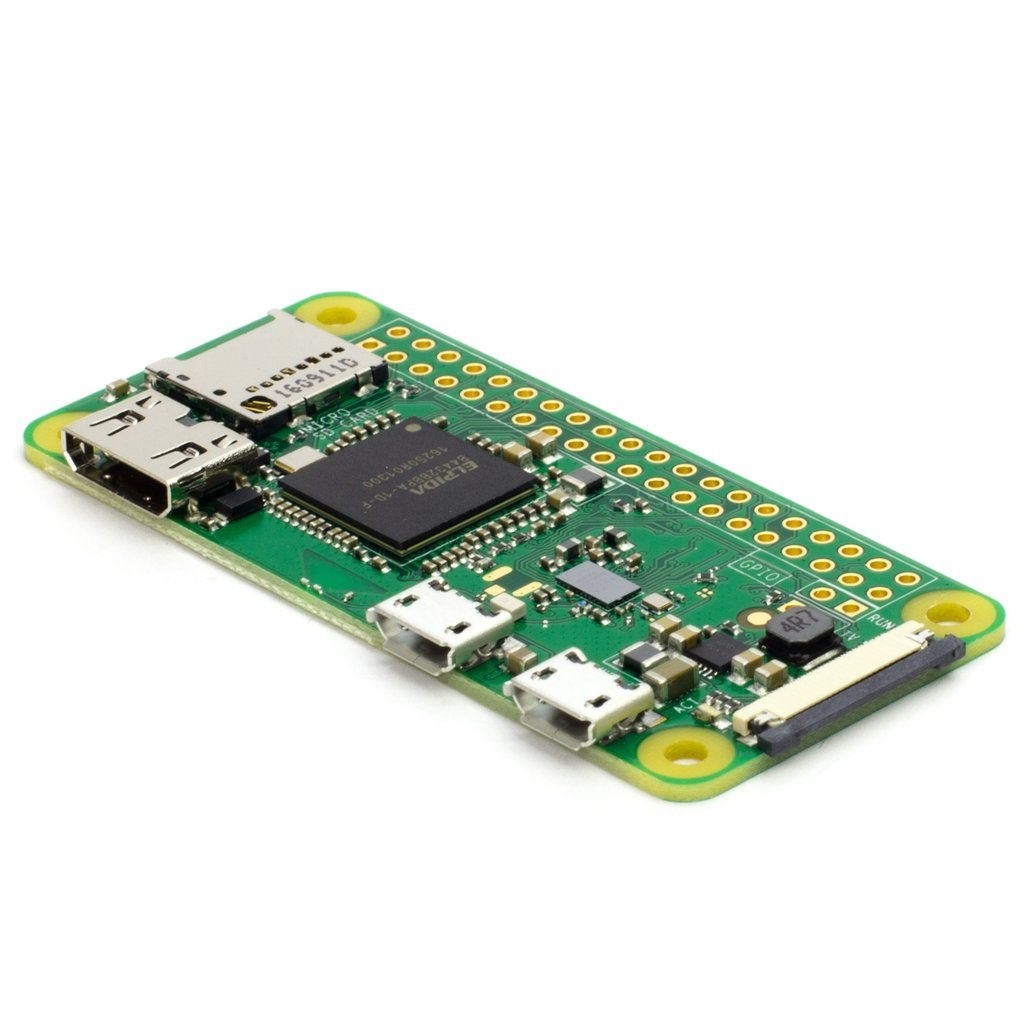
\includegraphics[width=0.5\textwidth]{images/raspberry_pi_zero_w.jpeg}
\end{figure}

Si vous avez besoin d'un micro-ordinateur, qu'il est possible de connecter
à des composants électroniques, le Raspberry Pi est la référence.
Cela dit, n'oubliez pas qu'il en existe différents modèles, et notamment
le Raspberry Pi Zero W, fait pour s'intégrer, se souder directement
sur une carte électronique.

\section{Micro-contrôleurs}

\begin{figure}[h]
\caption{Teensy 3.5}

\centering{}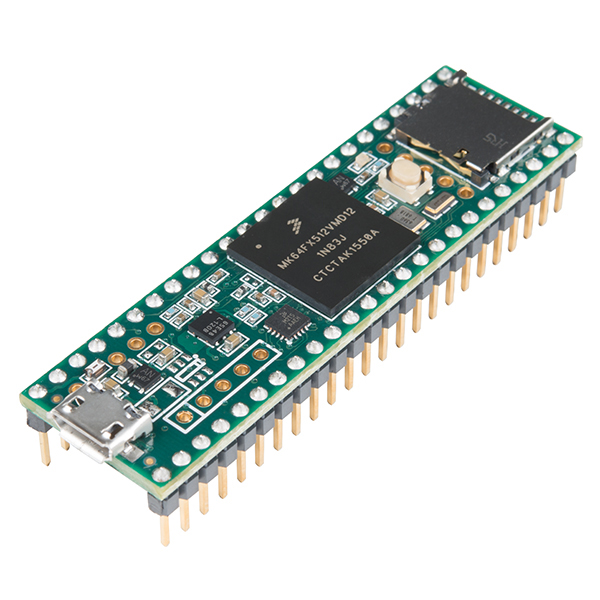
\includegraphics[width=0.5\textwidth]{images/teensy_3_5.jpg}
\end{figure}

Si vous avez à choisir un micro-contrôleur, je vous suggère de jeter
un oeil aux microcontrôleurs arduino-compatibles Teensy, que vous
pouvez trouver sur le site du fabricant : pjrc.com.

Par rapport aux cartes arduino, ils ont l'avantage d'utiliser des
signaux logiques en 3.3V (tout en étant 5V compatibles pour certains
modèles), d'avoir beaucoup plus de ports série, I2C, SPI... d'être
plus puissants à un meilleur rapport qualité prix. Ils sont faits
pour être soudés sur une carte en ''through hole'' et sont plus
compacts.

\section{Convertisseur USB-série}

\begin{figure}[h]
\caption{Convertisseur USB-série}

\centering{}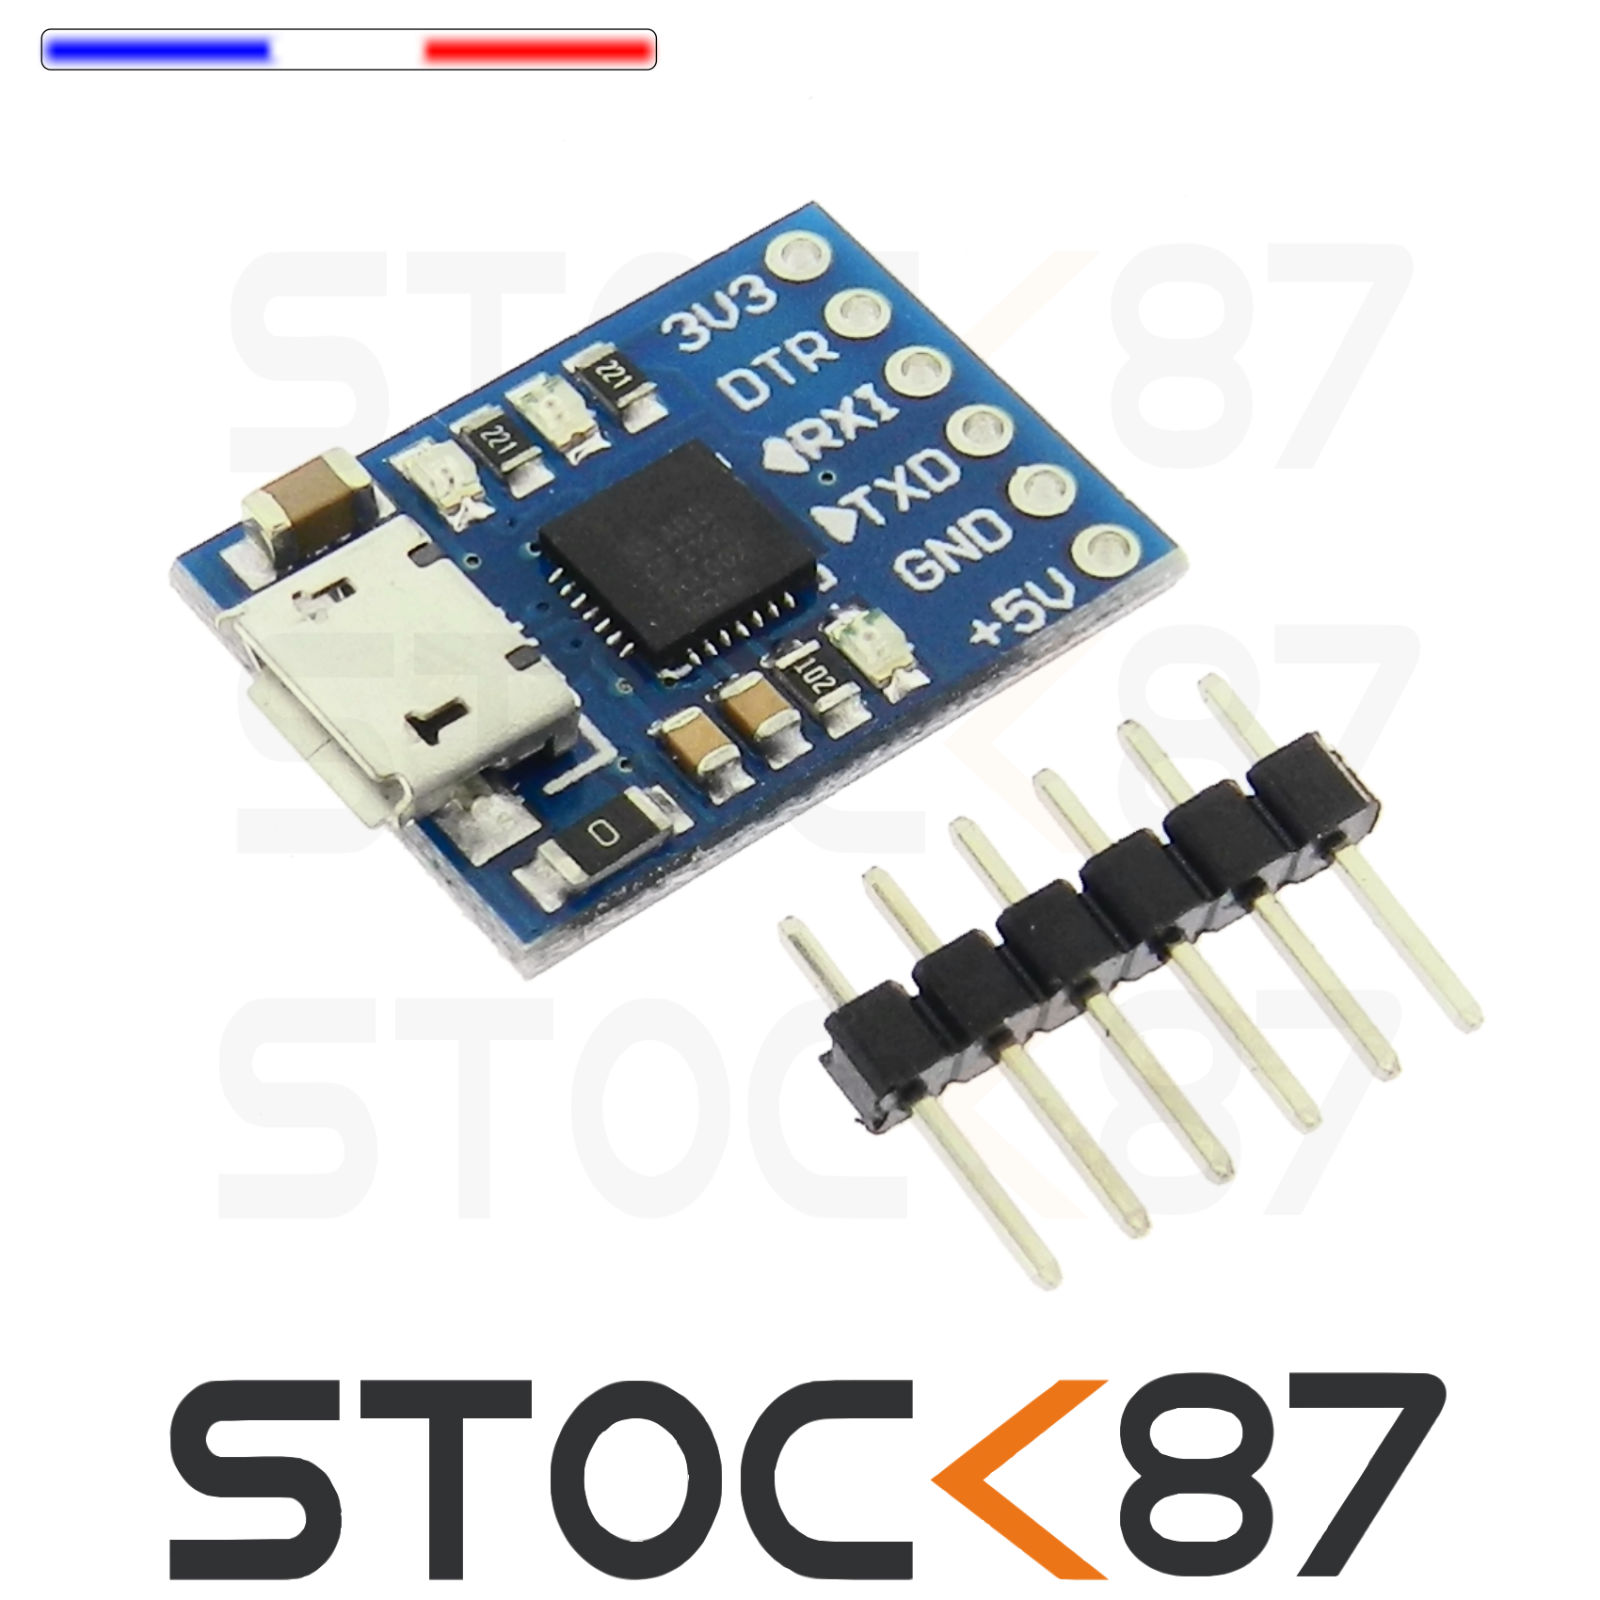
\includegraphics[width=0.4\textwidth]{images/usb_serie.png}
\end{figure}

Ce composant bien pratique permet de connecter un port USB à un port
série. On peut en trouver notamment dans la boutique du vendeur ebay
electron-discount, qui est un très bon vendeur situé en France pour
de petits composants électroniques.

\section{La centrale inertielle (IMU)}
Afin de pouvoir connaître l'attitude du bateau (roulis,tangage et cap), une centrale inertielle est utilisée: la VN-100 de Vectornav.

Elle est composé de:
\begin{description}
\item[3 accéléromètres:]Mesurent les accélérations selon les axes X, Y et Z. Ils mesurent toutes les forces sauf la gravité.
\item[3 gyromètres:]Mesurent les vitesses de rotations selon les axes X, Y et Z. Il faut faire attention car ils possèdent un biais qui évoluent en fonction du temps et fait dériver les mesures d'angles obtenues par intégration.
\item[3 magnétomètres:]Mesures le champ magnétique selon les 3 axes X, Y et Z. Les mesures sont très susceptibles à l'environnement autour des capteurs. Les métaux alentours modifient le champ magnétique et donc les mesures.
\end{description}

Les mesures obtenues avec ces capteurs sont filtrés avec un filtre de Kalman. Ainsi, l'IMU nous donne directement les données traitées.

\begin{figure}[h]
	\begin{center}
		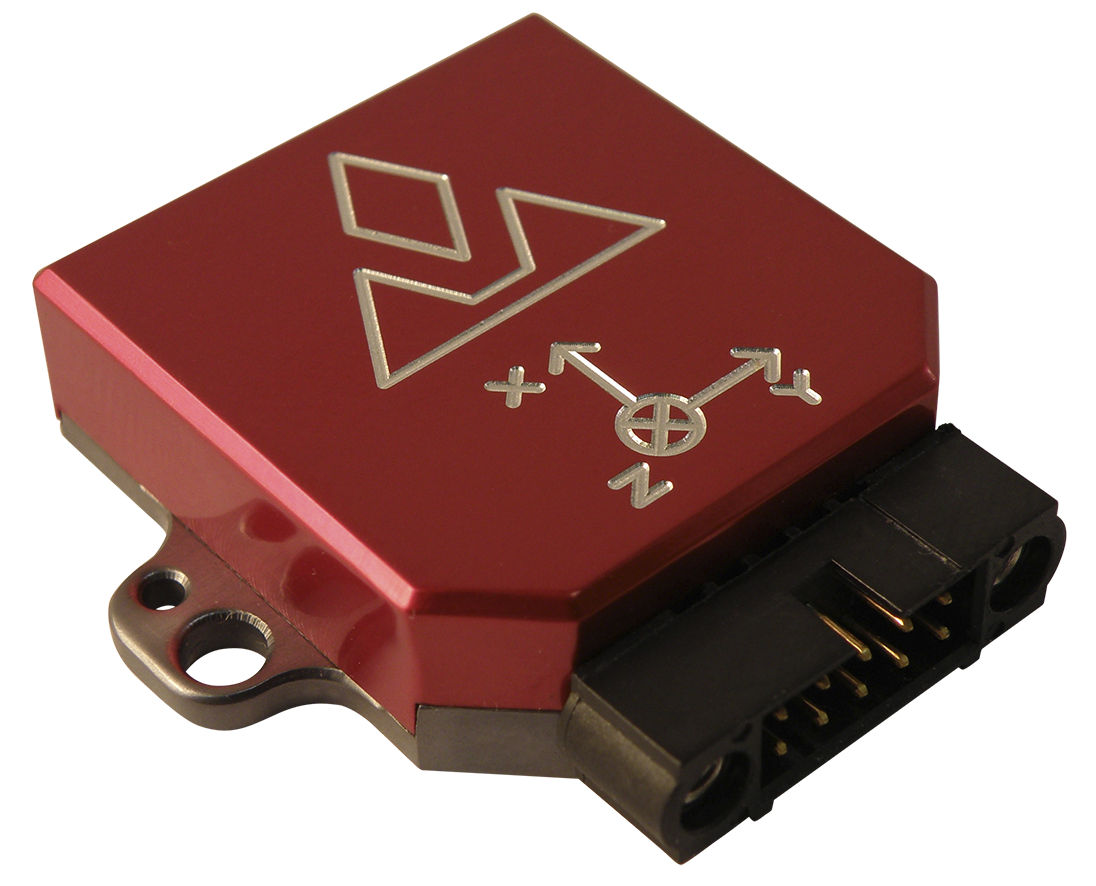
\includegraphics[width=0.5\textwidth]{images/IMU.jpg}
		\caption{IMU VN100 de Vectornav}
	\end{center}
\end{figure}

\section{Le récepteur GPS}
Un récepteur GPS RTK est utilisé afin de connaître la position du bateau. Un GPS RTK permet d'obtenir une précision de l'ordre du centimètre contrairement aux GPS conventionnels. Nous utilisons le GPS RTK de EMLID.

\begin{figure}[h]
	\begin{center}
		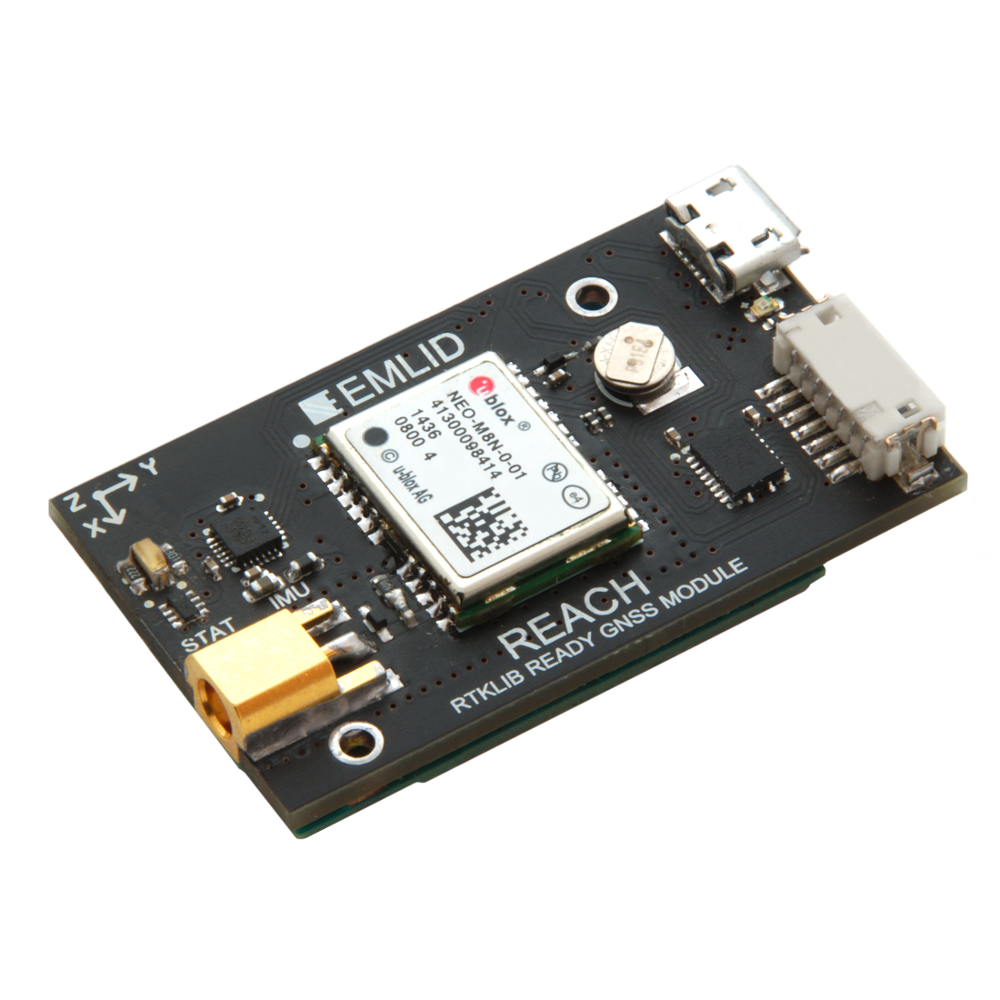
\includegraphics[width=0.5\textwidth]{images/gps.png}
		\caption{Récepteur GPT RTK de Emlid}
	\end{center}
\end{figure}

Le GPS RTK a besoin d'une station au sol dont on connait parfaitement la position. Ainsi, cette station va pouvoir mesurer les altérations qu'on subit les signaux des satellites en traversant l'atmosphère. Cette station va ensuite envoyer les corrections obtenus au récepteur GPS.

Nous possédons 2 stations GPS RTK. Une sert de base au sol de référence et l'autre est embarquée sur le bateau. Il est aussi possible de connecter le récepteur GPS à des stations de corrections locales.

Pour utiliser cette technologie sans avoir besoin d'installer notre
propre station GPS de référence à quai, nous avons pu obtenir des
identifiants pour nous connecter par internet (protocole NTRIP) à
certaines stations de correction du réseau rgp-ip maintenu par l'IGN
(rgp-ip.ign.fr).

Voici les infos sur les deux serveurs auxquels nous avons accès:
\begin{enumerate}
\item RGP-IP : rgp-ip.ign.fr, port 2101 ou 80, format RTCM3, login : jbarber, mdp : dM76F4zg\$\$

\item EUREF-IP : euref-ip.be, port 2101, format RTCM3, login : hydomines, mdp : pietrocontest
\end{enumerate}

S'il est imposible de se connecter à rgp-ip avec le reach, il est possible d'utiliser cette application android : https://play.google.com/store/apps/details?id=com.lefebure.ntripclient qui peut se connecter et transmettre les corrections par bluetooth au Reach.

\section{Le LIDAR}
Un LIDAR  (Laser Detection And Ranging) permet de mesurer la distance d'un point en face de lui. Ainsi, en le faisant tourner, on peut obtenir la distance de tous les objets l'entourant dans un plan. 

Nous avons le RPLIDAR A3 de Slamtec. Nous l'utilisons en combinaison avec une gimbal afin de détecter les obstacles en surfaces.

\begin{figure}[h]
	\begin{center}
		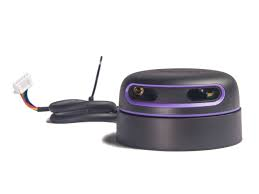
\includegraphics[width=0.5\textwidth]{images/LIDAR.jpg}
		\caption{RPLIDAR A3 de Slamtec}
	\end{center}
\end{figure}

\chapter{Composants électriques}

\section{Interrupteurs}

Il est souvent pratique d'installer les interrupteurs au travers de
la cloison d'un boîtier étanche. Ces interrupteurs doivent donc aussi
être étanches et on veillera à leur indice de protection.

\begin{figure}[h]
\caption{Interrupteur d'arrêt d'urgence (gauche) / Interrupteur à bascule (droite) }

\centering{}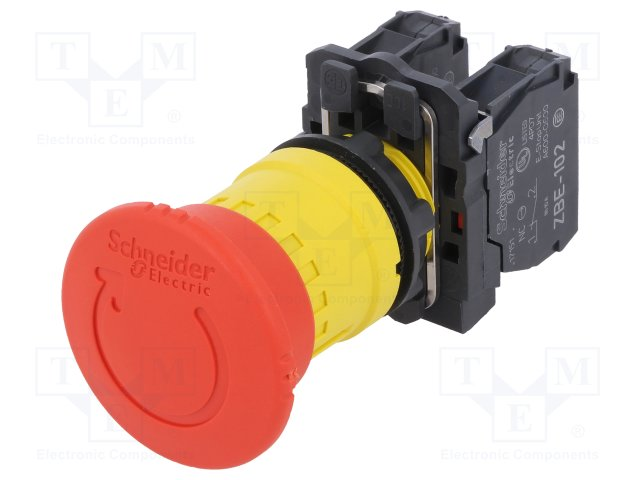
\includegraphics[width=0.5\textwidth]{images/arret_urgence}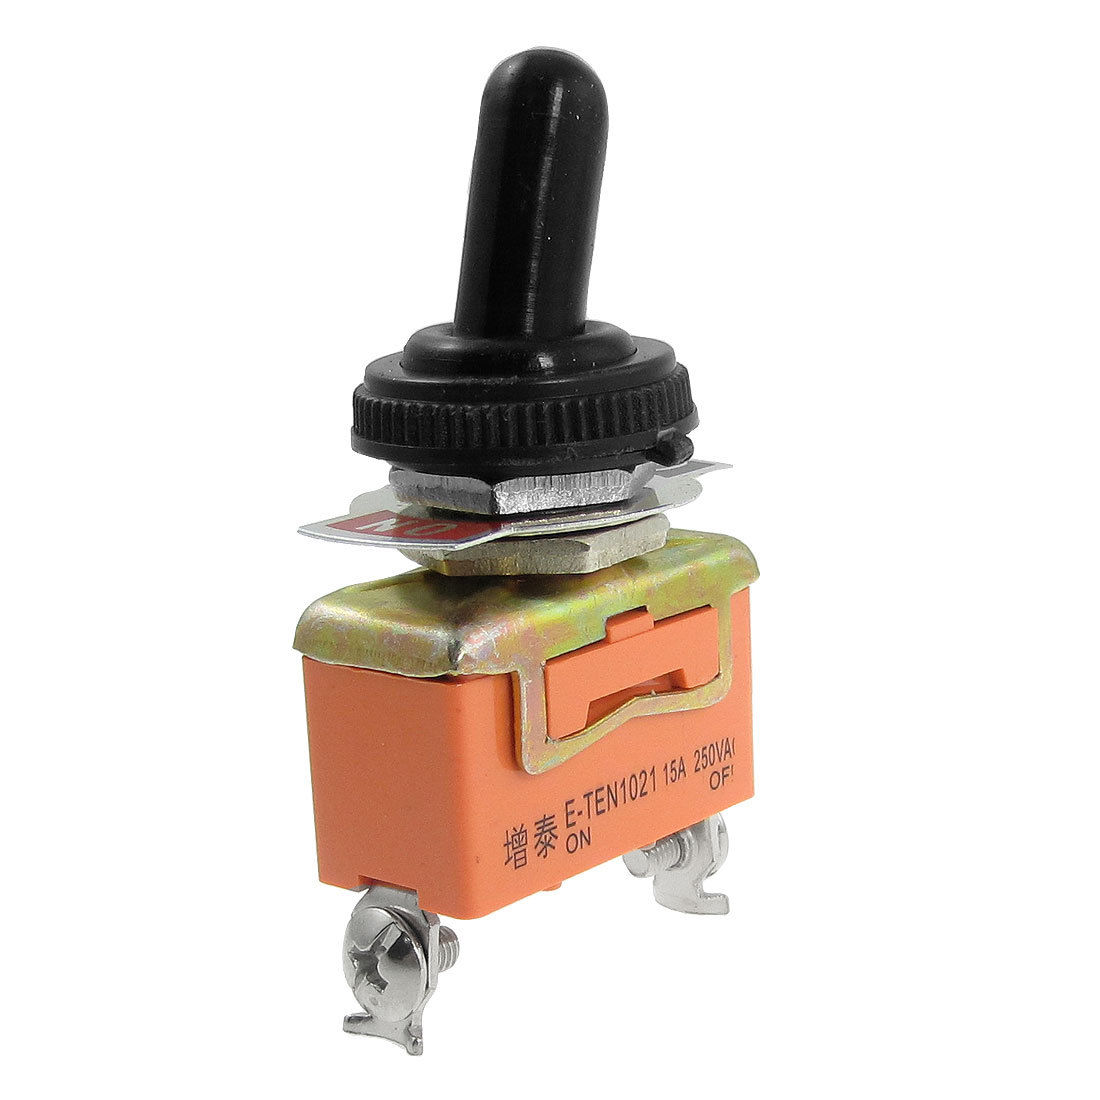
\includegraphics[width=0.5\textwidth]{images/interr_etanche}
\end{figure}

Ce type de bouton d'arrêt d'urgence est bien pratique puisqu'il permet
de gérer deux circuits à la fois, l'un NF (normalement fermé) et l'autre
NO (normalement ouvert). On a souvent besoin des deux car si on peut
couper l'alimentation du BEC en cas d'urgence (circuit normalement
fermé), il ne faut pas mettre d'interrupteur entre la batterie et
le variateur (ceci créerait des étincelles). Pour éteindre le variateur,
on met en contact deux de ses fils ce qui lui envoie un signal logique
d'arrêt (circuit normalement ouvert ici). On peut trouver ce type
d'interrupteur chez le fournisseur tme.eu. 

Pour les interrupteurs classiques, le plus simple est de prendre de
petits interrupteurs à bascule avec capuchon caoutchouc assurant l'étanchéité.
On peut notamment en trouver sur ebay.

Ces deux types d'interrupteur se montent facilement à travers une
cloison, après avoir percé un trou du bon diamètre.

\section{Fusibles et porte-fusibles}

Le fusible sur le circuit du variateur et son porte-fusible sont fournis
par la compétition. Il est cependant nécessaire d'installer d'autres
fusibles, notamment sur les circuits que nous réalisons nous-mêmes.
Pour ce faire, le mieux est d'utiliser des fusibles rapides (c'est
à dire qu'ils sautent rapidement en cas de trop forte intensité) cylindriques
au format 5x20, faciles à trouver. On trouve facilement des kits de
fusibles de ce type sur amazon en y recherchant ''fusible verre''
par exemple.

Afin d'intégrer ces fusibles à nos circuits électriques, on peut utiliser
deux types de porte fusibles :

\begin{figure}[h]
\caption{Porte fusible ''through hole'' pour carte électronique (gauche)
ou à souder à des fils (droite)}

\centering{}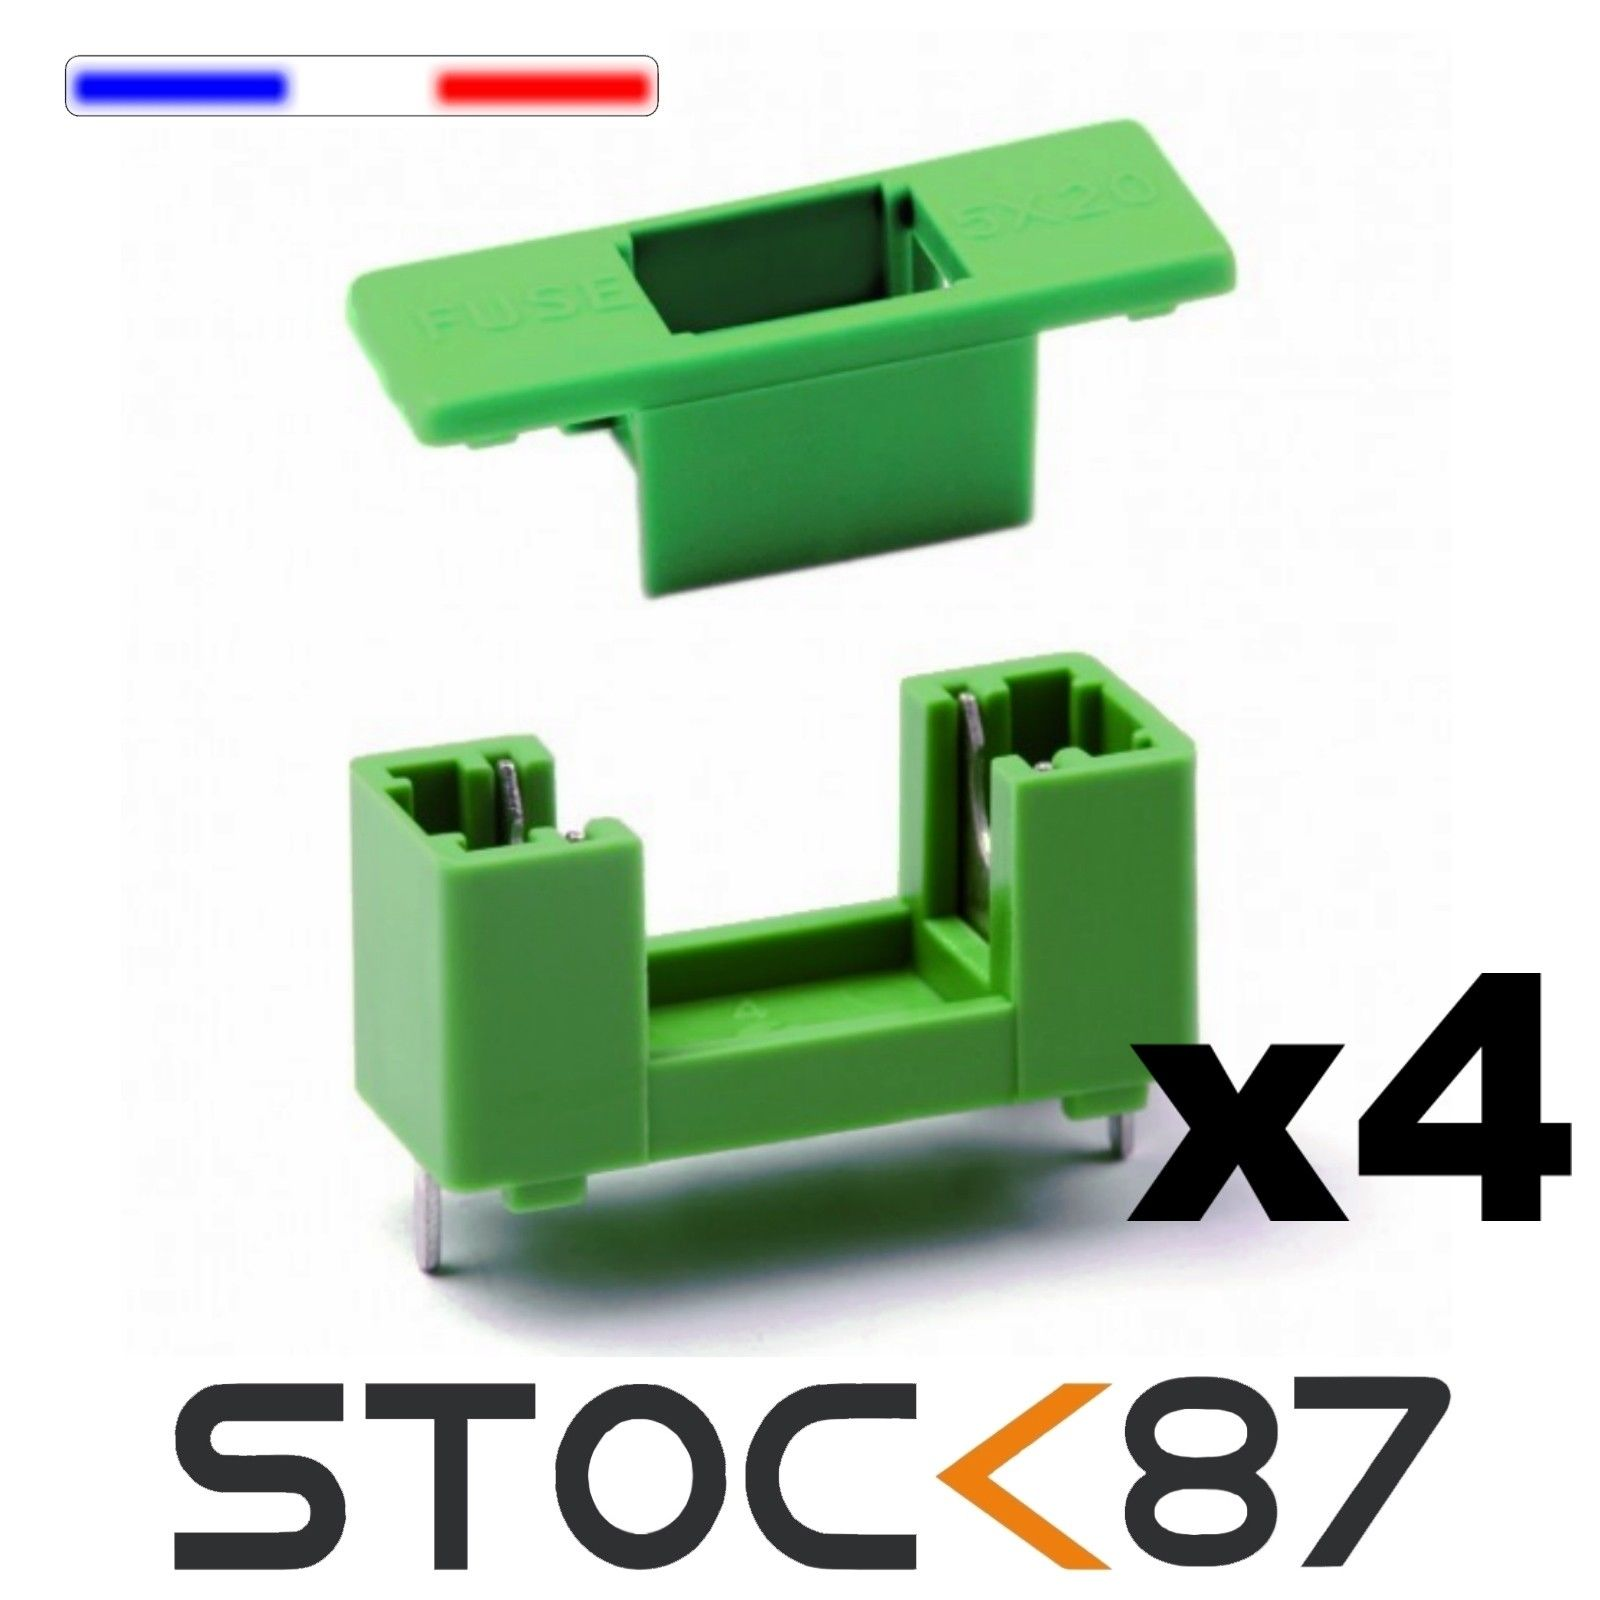
\includegraphics[width=0.5\textwidth]{images/porte_fusible_th.jpg}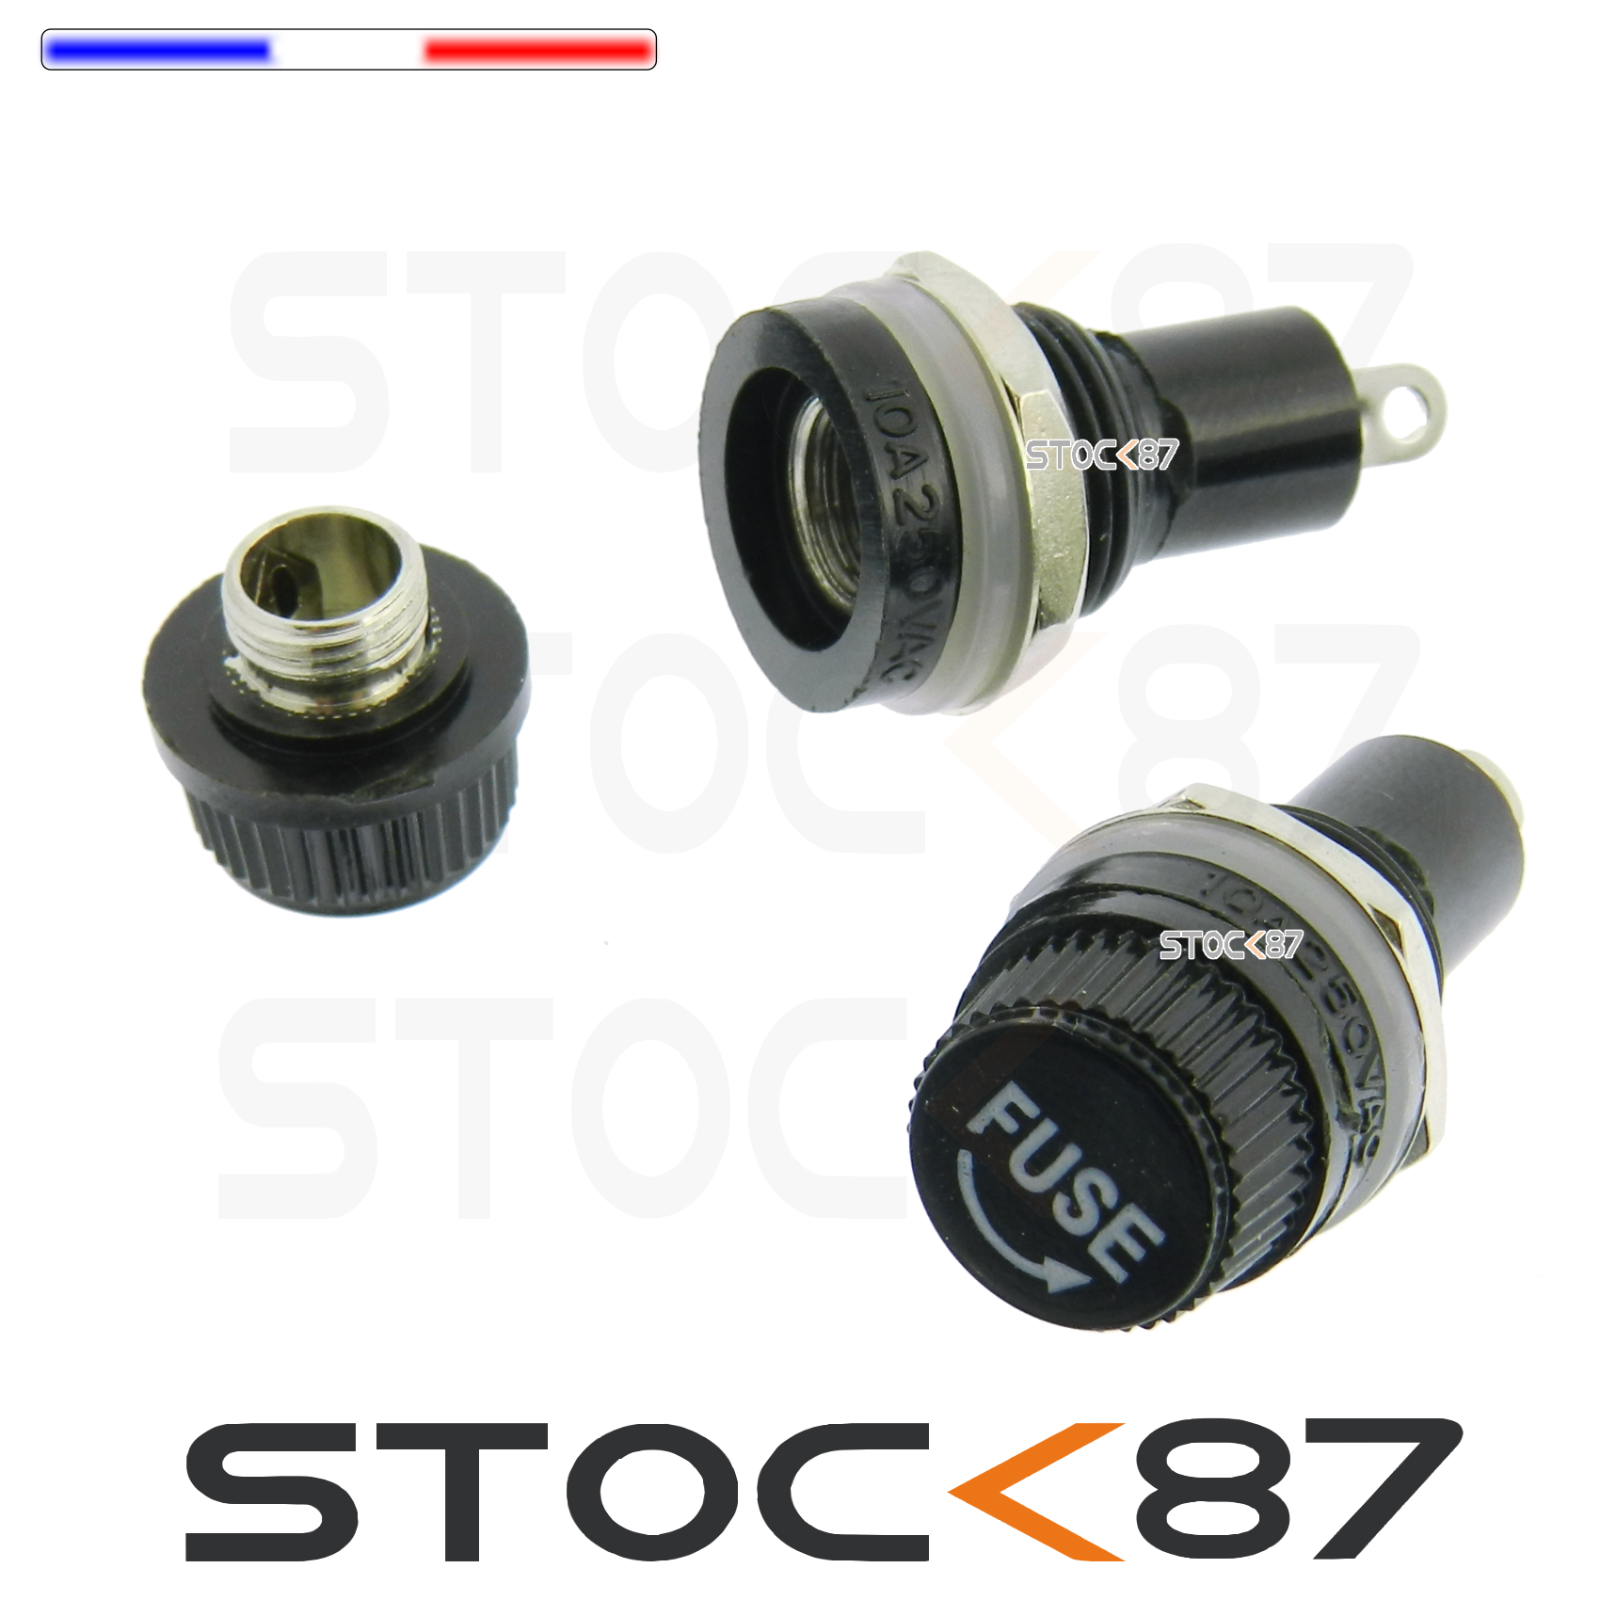
\includegraphics[width=0.5\textwidth]{images/porte_fusible_fil.png}
\end{figure}

Vous pourrez notamment trouver ces produits sur la boutique ebay du
vendeur electron-discount.

\section{Batteries}

Bien que les batteries soient fournies pendant la compétition, il
est très utile d'avoir des batteries de test pendant l'année. La solution
la plus simple pour obtenir une batterie de 37V comme celle de la
compétition est de se tourner vers des batteries LiPo (lithium polymère).
Il faut assembler 10 cellules LiPo en série (3.7V chacune) pour atteindre
les 37V. On trouve facilement des batteries 5S (ce qui veut dire 5
cellules en série) sur hobbyking, et il est donc possible d'en acheter
deux et les assembler en série. Prenez si possible des batteries munies
de connecteurs XT-90, qui sont les connecteurs des batteries de la
compétition.

Avant l'achat et l'utilisation de batteries LiPo, renseignez vous
sur cette technologie de batterie, les critères pour choisir une batterie,
comment elles s'utilisent et les dangers qu'elles représentent. Trop
charger ou décharger une LiPo, ou le faire trop vite (courant trop
important) est dangereux !

Vous aurez aussi besoin d'un chargeur spécifique aux batteries LiPo,
qui permet l'équilibrage de la charge des différentes cellules.

Pour l'utilisation des LiPo, je vous conseille d'acheter des sacs
pour batteries LiPo (visant à limiter les dégâts si la batterie prend
feu ou explose), ainsi que des indicateurs de tension, qui se branchent
sur les connecteurs d'équilibrage des LiPo et permettent de vérifier
leur tension pendant leur utilisation. On peut aussi fixer un seuil
limite (cellule par cellule) en dessous duquel une alarme retentit,
ce qui permet de ne pas trop décharger la batterie (ce qui est très
dangereux).

\chapter{Matériel pour réaliser des circuits}

\section{Perfboards}

\begin{figure}[h]
\caption{Perfboard (gauche) / Perma-proto board (droite)}

\centering{}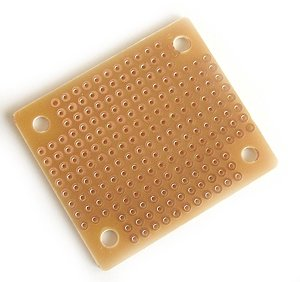
\includegraphics[width=0.5\textwidth]{images/perfboard}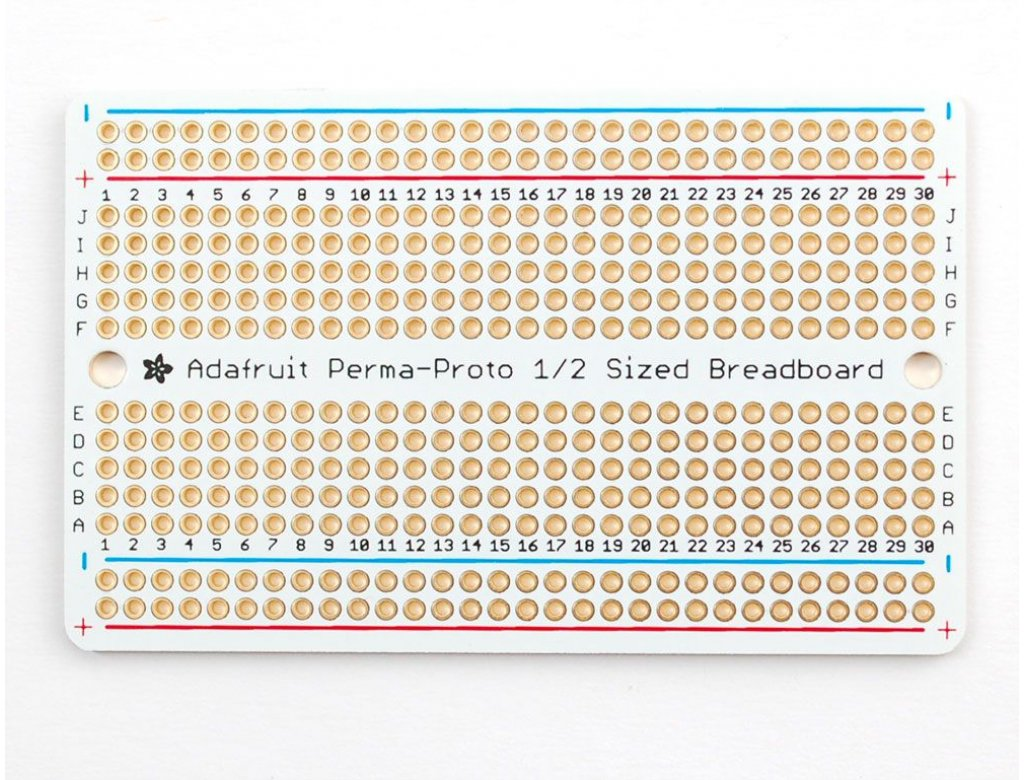
\includegraphics[width=0.6\textwidth]{images/perma_proto_board.jpg}
\end{figure}

La façon la plus propre de réaliser des circuits électroniques est
de rassembler les composants sur des cartes. Il est possible de le
faire à la main, sans avoir à faire fabriquer un circuit imprimé.
Pour cela, on utilise ce que les anglophones appellent des ''perfboards'',
qui sont des cartes faites pour y souder des composants ''through
hole'' ainsi que des fils et y réaliser des circuits. En français,
le terme consacré est carte ou platine de prototypage et on en trouve
facilement sur tous les sites d'électronique.

Une variante intéressante est la gamme de ''perma-proto boards''
conçue par Adafruit. Il s'agit de perfboards où certaines connexions
électriques sont déjà réalisées, reprenant le schéma de connexion
d'une breadboard (googlez breadboard si vous ne connaissez pas le
terme).

L'immense majorité de ces platines possède un espacement entre trous
de 2.54mm (0.1 inch), ce qui est l'espacement standard entre pins
pour les composants ''through hole'', et permet donc d'y souder
la plupart de ces composants.

\section{Faire fabriquer un circuit imprimé ?}

Si la perfboard permet déjà de réaliser des circuits électriques plus
propres, le niveau ultime est de faire fabriquer un circuit imprimé,
dans lequel les connexions électriques sont imprimées sur la carte
(sur un certain nombre de couches), ce qui fait qu'il ne reste plus
qu'à souder les composants ''through hole'' pour obtenir tous les
circuits. Si vous ne voyez pas bien ce qu'est un circuit imprimé,
lisez l'article intitulé ''PCB Basics'' sur le site de sparkfun.

Si la plupart des logiciels de conception sont assez difficiles à
prendre en main, il en existe un très simple qui est amplement suffisant
pour des besoins basiques (c'est à dire faire de la perfboard améliorée
en gros) : Fritzing. Tous ce que vous avez à faire grosso modo est
de définir la taille de votre PCB (printed circuit board, c'est à
dire circuit imprimé), à positionner dessus les trous pour les connexions
aux composants ''through hole'' (grâce au composant via du logiciel)
et à les relier entre eux. Vous pouvez aussi ajouter du texte, des
logos sur votre carte ou placer des trous de fixation par exemple.

\begin{figure}[h]
\caption{Aperçu du logiciel Fritzing}

\centering{}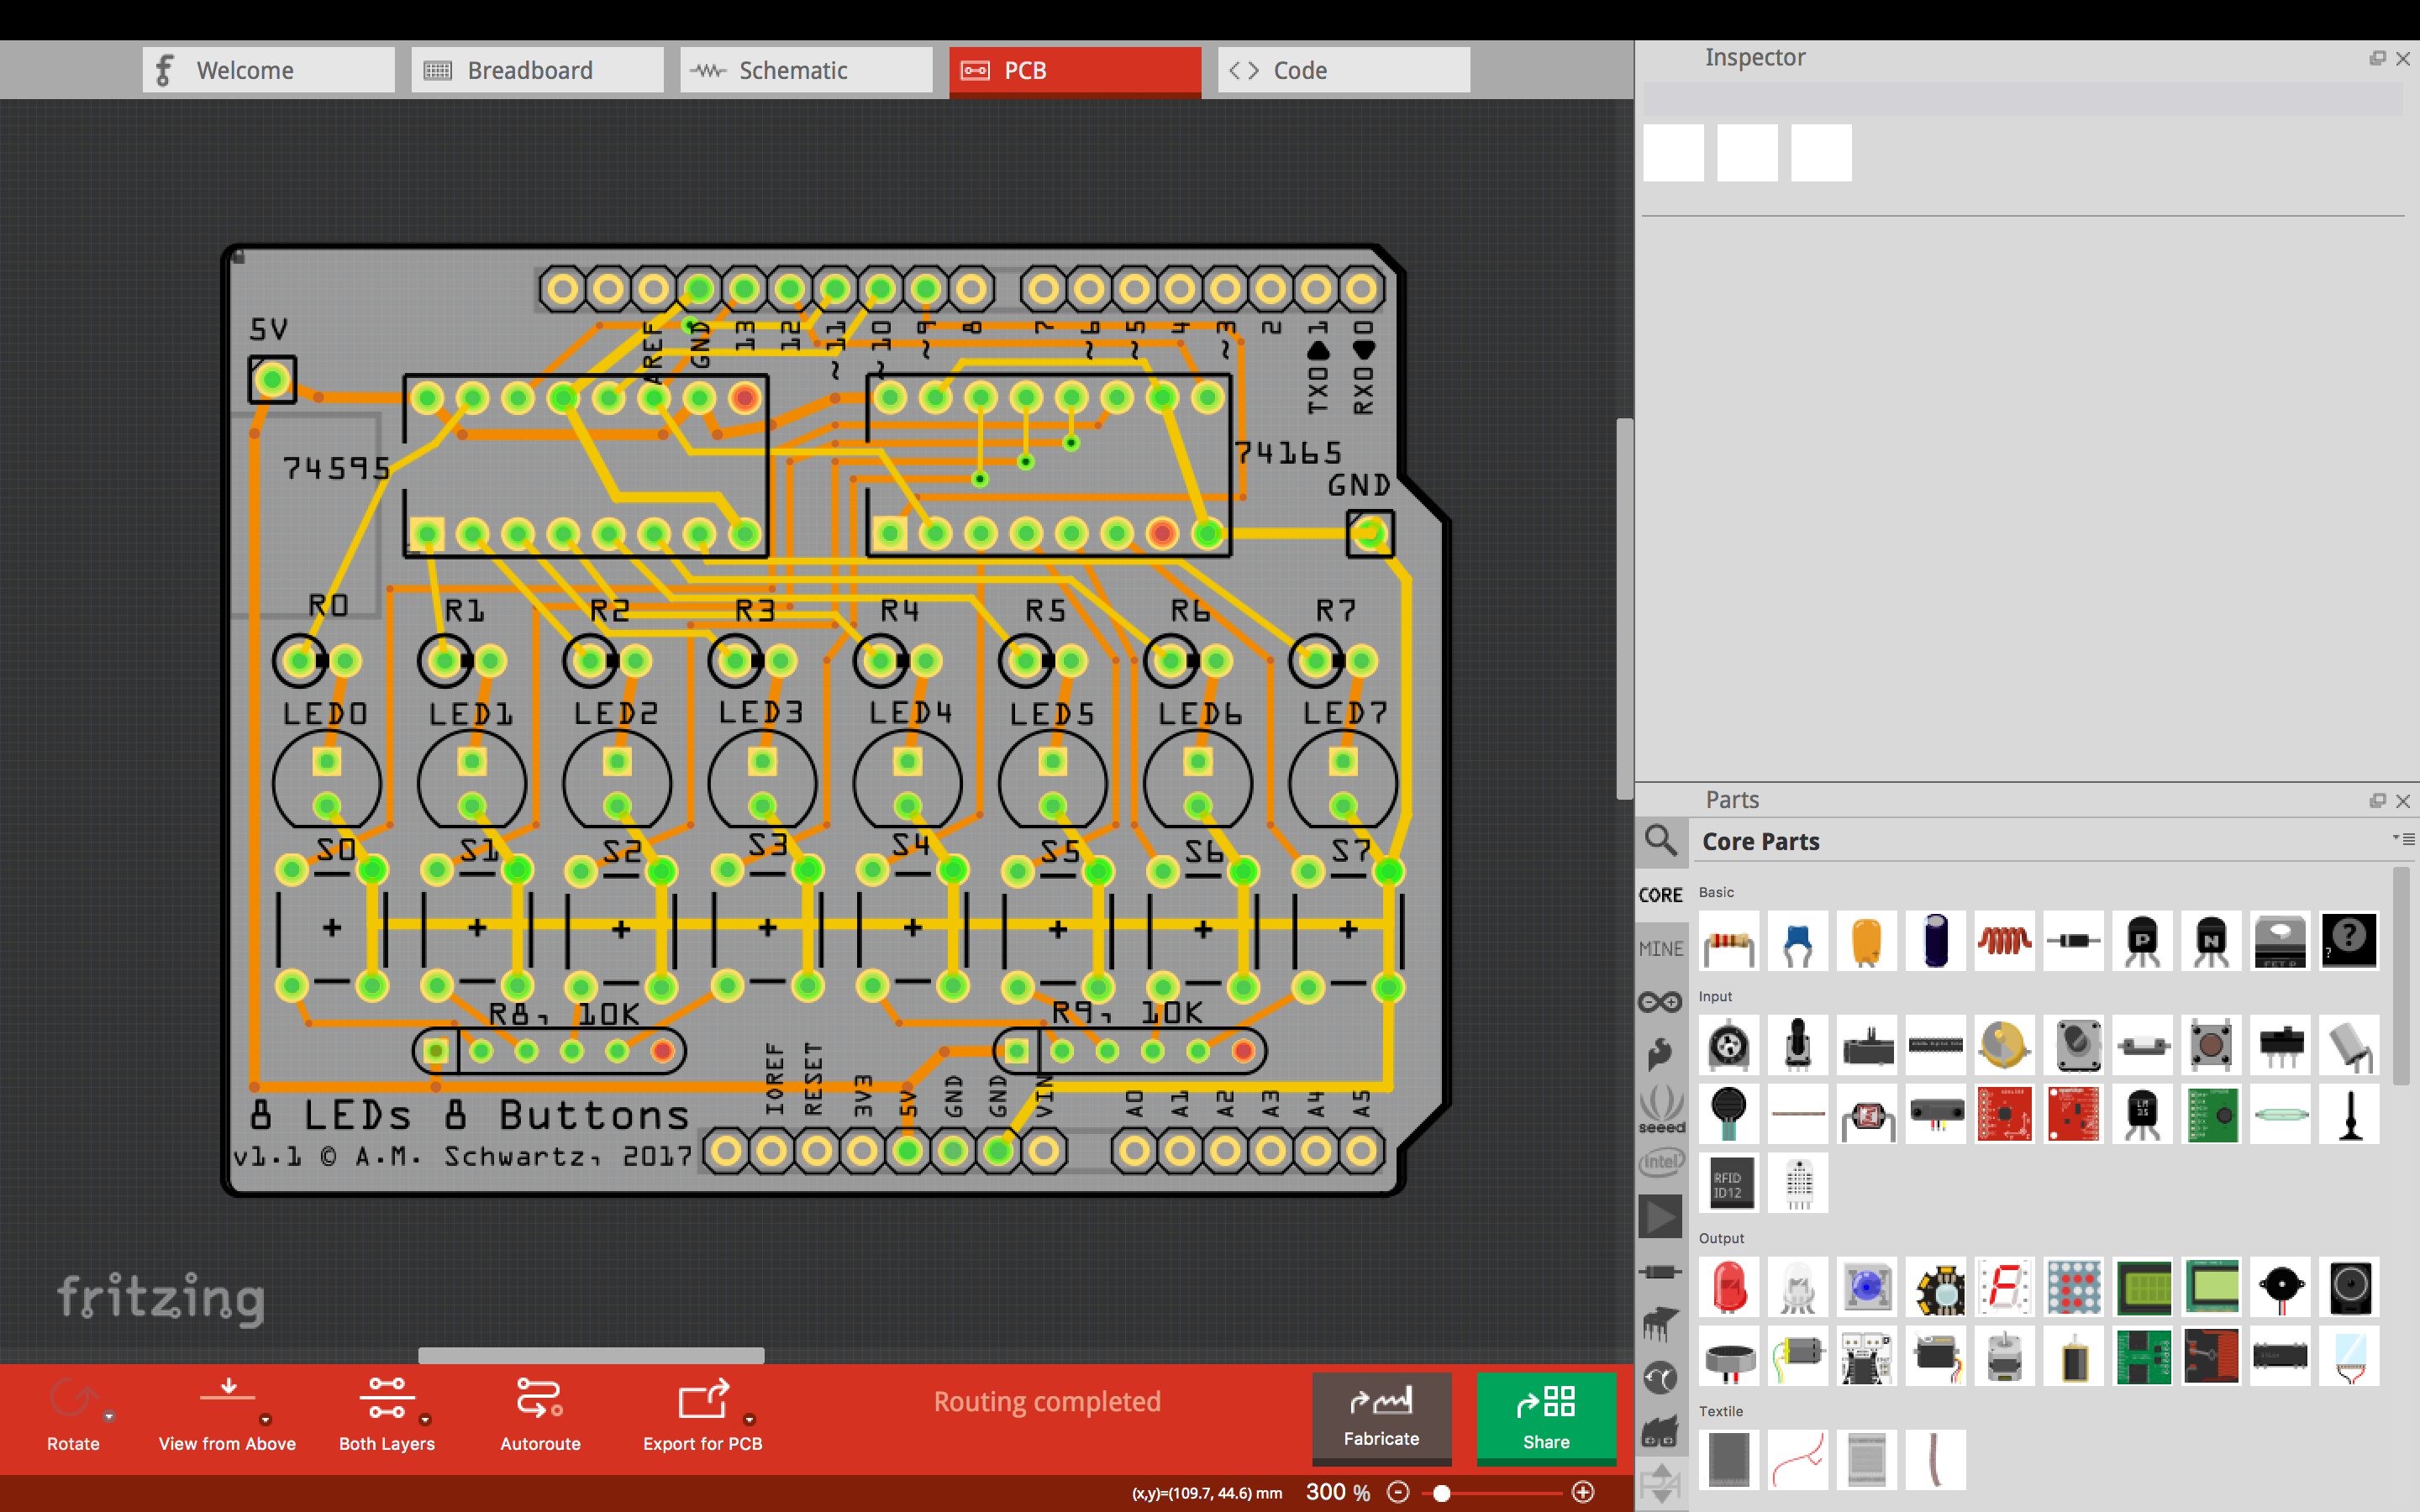
\includegraphics[width=1\textwidth]{images/fritzing}
\end{figure}

La difficulté consiste à tout bien dimensionner, que ce soit pour
les considérations mécaniques (vérifier que les pins rentrent dans
les trous ...etc), électriques (calculer l'intensité max que permettent
vos connexions, espacer assez les différentes connexions ...etc),
ou les contraintes imposées par le fabricant, puisque tout design
n'est pas réalisable (si vous demandez des espacements trop faibles
entre différents trous par exemple, mais en pratique les problèmes
arrivent pour des designs vraiment compliqués). L'utilisation du logiciel
est un jeu d'enfant (d'ailleurs il a en partie été pensé pour des
enfants, n'hésitez pas à trouver quelques tutos sur internet), mais
le logiciel vous permet quand même d'exporter votre design sous la
forme de ''Gerber files'', ce qui est le standard de l'industrie
pour la fabrication de circuits imprimés.

Une fois ces fichiers obtenus, il y a plein de sites chinois qui peuvent
fabriquer votre design pour un prix ridiculement bas (quelques dollars),
le principal coût étant les frais de port (attention aux délais de
livraison aussi). Le meilleur d'entre eux est JLC PCB, qui offre un
service impeccable au meilleur prix (fabrication en 2 jours ouvrés
et livraison en 5 jours ouvrés en choisissant le transporteur DHL).

N'hésitez pas à utiliser cette méthode, c'est vraiment simple, pas
cher et ça permet d'avoir des circuits d'une qualité incomparable.

\section{Connecteurs Dupont et JST}

Les connecteurs entrent en jeu quand il s'agit de connecter un circuit
à un composant externe ou à un autre circuit. J'ai principalement
travaillé avec deux types de connecteurs : Dupont et JST.

\begin{figure}[h]
\caption{Connecteurs Dupont femelle (gauche) / Rangée de pins (droite)}

\centering{}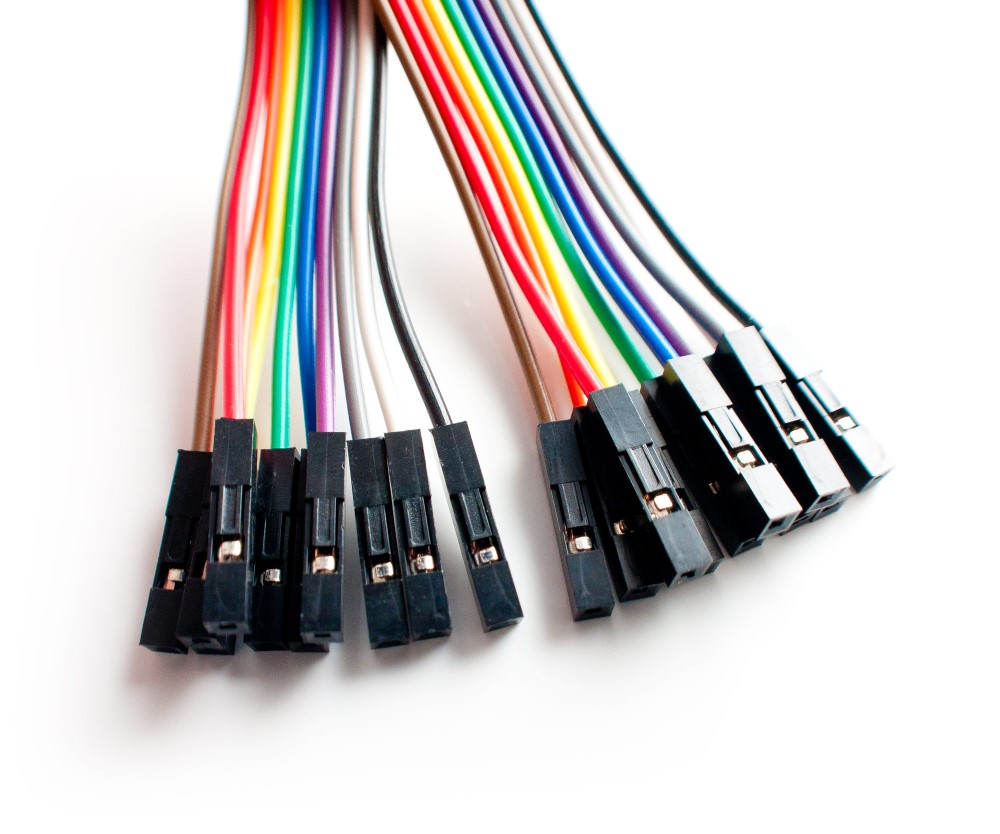
\includegraphics[width=0.5\textwidth]{images/dupont_femelle.jpg}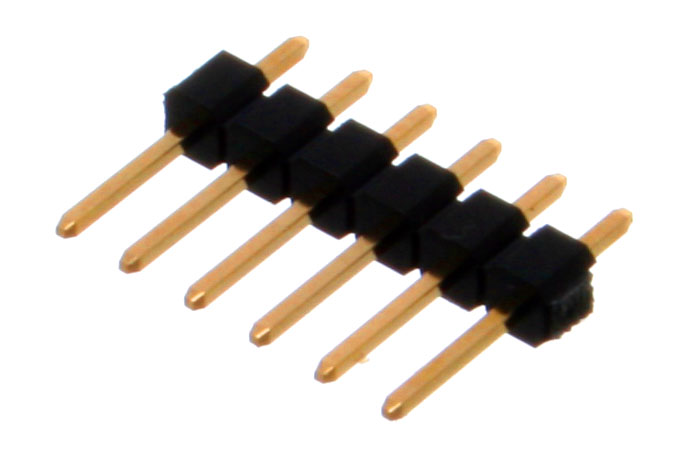
\includegraphics[width=0.5\textwidth]{images/pin_header.jpg}
\end{figure}

Le plus grand avantage des Dupont est qu'ils sont extrêmement courants,
on trouve facilement des cables male-femelle, femelle-femelle ...etc
(tout ce que vous voulez), et surtout que le connecteur Dupont mâle
n'est rien d'autre qu'un pin, il n'y a rien de plus simple !

Du coup, vous pouvez simplement souder une rangée de pins (pin headers
en anglais, barrette mâle en français) à votre carte électronique
et y brancher des cables Dupont qui pourront faire la liaison avec
d'autre circuits ou composants.

Niveau inconvénients, les connecteurs Dupont ne sont pas prévus pour
des courants très importants et la liaison mécanique entre le pin
et le connecteur femelle saute assez facilement.

Pour les deux problèmes cités, les connecteurs JST sont une amélioration,
mais demandent plus d'effort puisqu'ils demandent un sertissage.

\begin{figure}[h]
\caption{Connecteur JST}

\centering{}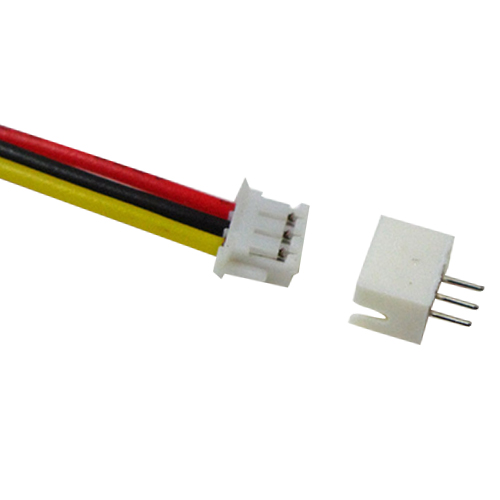
\includegraphics[width=0.5\textwidth]{images/jst}
\end{figure}

Il existe différents formats (2 pin, 3 pin, ...etc) et le mieux est
souvent d'acheter un kit jst (on en trouve plein sur amazon), qui
comprendra des connecteurs male et femelle de différents formats et
de quoi les sertir.

\section{Fil électrique pour hautes intensités}

La documentation technique du concours impose certaines sections minimales
de fil électrique pour les circuits de puissance (alimentation du
variateur et du moteur). Les sections de fil électrique sont le plus
souvent mesurées en AWG (selon l'American Wire Gauge, cf wikipedia),
ce qui correspond à une aire. Vous pouvez trouver des tableaux reliant
l'AWG d'un fil à l'intensité maximale recommandée (qui est aussi fonction
du nombre de brins notamment).

Pour trouver des fils de grande section pour les circuits de puissance,
le mieux est d'utiliser le matériel utilisé dans les installations
électriques domestiques, et donc de se rendre dans un magasin de bricolage.

Un bon choix pour les circuits de puissance est de prendre du fil
AWG 10 (6 mm ) pour l'alimentation du variateur et
du fil AWG 12 (4 mm ) pour les fils reliant le variateur
au moteur (vérifier en fonction du réglement qui peut évoluer).

\section{Connecteurs haute puissance}

Le choix des connecteurs pour les circuits de haute puissance est
très important, c'est pourquoi le réglement du concours l'impose généralement
(lisez le bien). Il est notamment primordial de toujours fermer ou
ouvrir le circuit d'alimentation du variateur au niveau d'une paire
de connecteurs anti-étincelles (en suivant la procédure particulière
de connexion/déconnexion pour ce connecteur) afin d'éviter la formation
d'arcs électriques. Hormis cette question d'étincelles, les connecteurs
ont aussi des intensités maximales et il faut donc bien les dimensionner.
N'hésitez pas à aussi apprendre à les souder correctement, ce qui
peut demander un peu de technique.

Les connecteurs imposés par la compétition sont souvent des connecteurs
courants en modélisme, que vous pourrez donc trouver sur un site de
modélisme comme hobbyking.

\section{Wago}

Il est parfois très utile de pouvoir connecter deux fils de haute
puissance de façon non définitive, en ayant la possibilité de défaire
et refaire la connexion un grand nombre de fois.

\begin{figure}[h]
\caption{Wago à levier, max 4mm (gauche) / Wago pour fils
de grande section, max 6mm (droite)}

\centering{}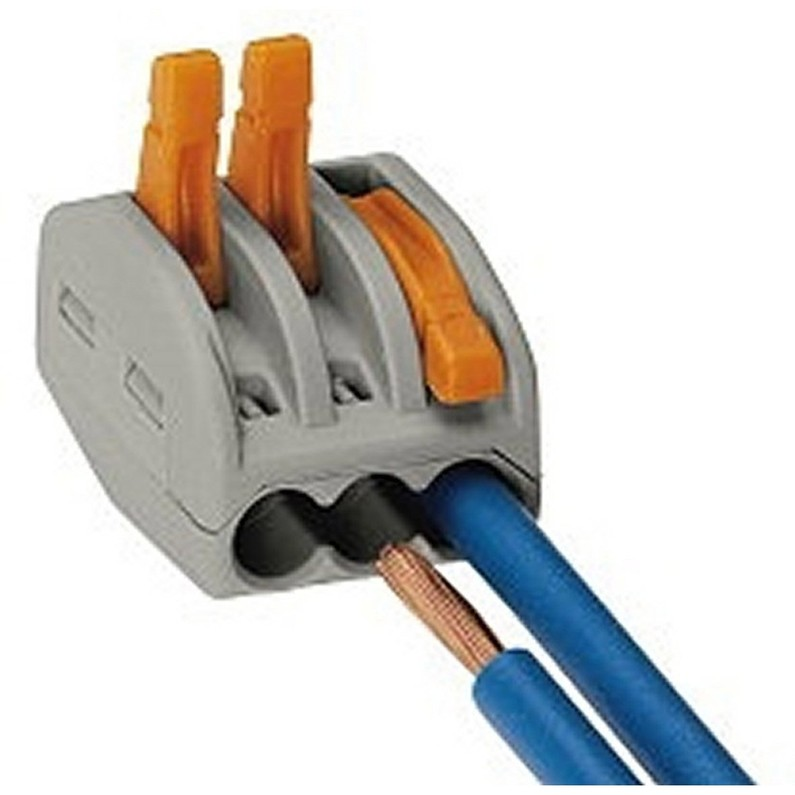
\includegraphics[width=0.5\textwidth]{images/wago_levier.jpg}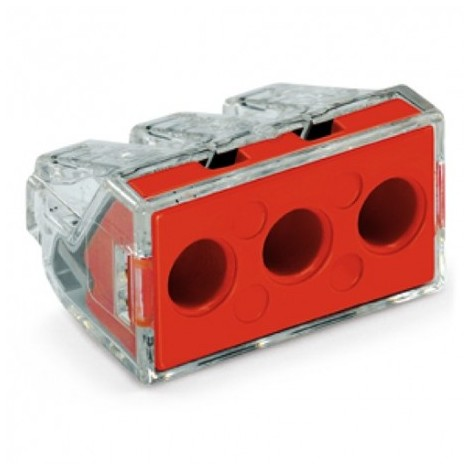
\includegraphics[width=0.5\textwidth]{images/wago_6mm2.jpg}
\end{figure}

Les électriciens utilisaient auparavant des dominos pour faire cela,
mais les wago (de la marque Wago) sont une alternative bien plus pratique
(connexion extrêmement robustes, bien plus rapide à faire et défaire).

Pour quoi faire si on a déjà des connecteurs et que l'on peut souder
les fils entre eux ? Déjà, en fonction de la qualité de vos soudures,
les wago peuvent permettre une connexion mécaniquement plus solide.
Ensuite, on a parfois besoin de faire passer des cables de haute puissance
d'un boîtier à un autre, et s'ils sont munis de gros connecteurs,
il peut être difficile de les faire passer à travers les sorties étanches
du boîtier, d'où l'intérêt de pouvoir faire et défaire la connexion
du fil aux connecteurs dans chacun des boîtiers.

Les wagos à levier se trouvent facilement en magasin de bricolage,
les wagos compatibles 6mm sont plus difficiles à
trouver, mais on en trouve sur amazon.

\chapter{Boîtiers étanches}

Pour les boîtiers étanches, je vous conseille vivement de les acheter
chez le fournisseur tme.eu, qui est sensiblement moins cher et offre
beaucoup plus de choix que d'autres fournisseurs. Vous les trouverez
dans la catégorie ''Boîtiers universels'', où vous pourrez utiliser
différents filtres pour trier parmi les quelques milliers de références.
Les principaux critères de choix sont :
\begin{enumerate}
\item la taille
\item la couleur du couvercle (voir contraintes du réglement)
\item l'indice de protection
\item la masse
\end{enumerate}

\chapter{Circuit de refroidissement}

Le variateur fourni par la compétition doit être refroidi par eau.
Il dispose de deux connexions rapides hydrauliques pour tubes de diamètre
extérieur 8mm. Ces connexions rapides sont également appelées ''push
fit fittings'', ''push in fittings'' ou ''quick fittings''. Elles
sont très simples à faire et défaire, vous pouvez chercher ''push
fit fitting'' sur youtube pour voir comment cela fonctionne.

Le plus simple est donc d'utiliser du tube nylon de diamètre extérieur
8mm et des composants tous munis de connexions rapides 8mm pour réaliser
le circuit de refroidissement. Il est possible de réaliser un circuit
ouvert, avec prise et lacher d'eau dans la mer, ou alors un circuit
fermé avec un réservoir d'eau et un échangeur eau-air extérieur pour
dissiper la chaleur accumulée par l'eau du circuit de refroidissement.
Dans tous les cas, les composants sont à peu près les mêmes, et je
vais les détailler un par un.

Les composants nécessaires à la réalisation d'un circuit de refroidissement
ne sont vraiment pas facile à trouver. J'ai tout de même trouvé un
site web anglais très intéressant où on trouve à peu près tout : https://www.advancedfluidsolutions.co.uk/
(AFS en abrégé).

\section{Tube nylon}

\begin{figure}[h]
\caption{Tube nylon (gauche) / Tube cutter (droite)}

\centering{}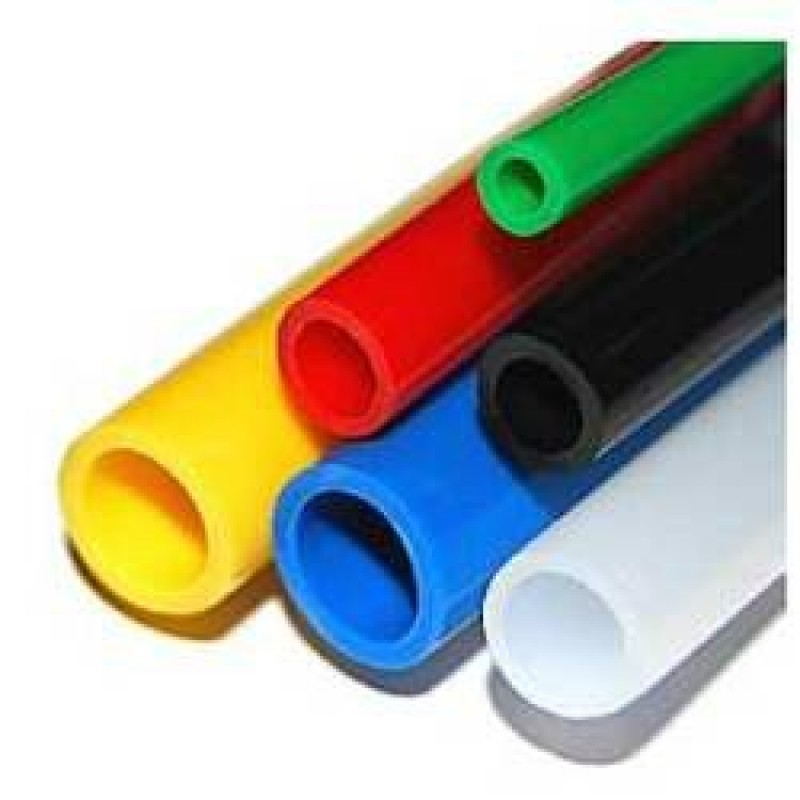
\includegraphics[width=0.5\textwidth]{images/nylon_tubing.jpg}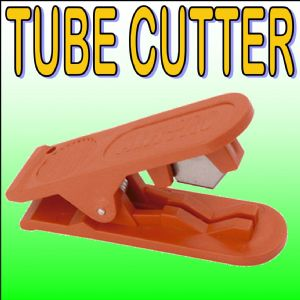
\includegraphics[width=0.5\textwidth]{images/tube_cutter.jpg}
\end{figure}

Veillez à prendre de la marge vis à vis de la longueur de tube, le
tube a tendance à partir assez rapidement et on peut se retrouver
avec pas mal de chutes. Pour couper correctement (et instantanément)
du tube nylon, il faut voir sous la main un ''tube cutter''.

Ces articles sont disponibles chez AFS (advanced fluid solutions).

Nous aurons besoin de faire passer ce tube à travers les parois de
boîtiers étanches, sans compromettre leur étanchéité ou causer de
fuites. Pour ce faire, le mieux est de se munir de ''bulkhead'',
ou passe-cloison, munis de connexions rapides 8mm. Vous pouvez en
trouver à bon prix chez RS dans la catégorie ''Pneumatic Bulkhead
Tube-to-Tube Adaptors''.

\begin{figure}[h]
\caption{8mm push fit bulkhead}

\centering{}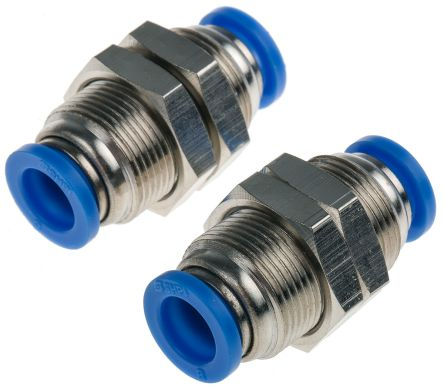
\includegraphics[width=0.4\textwidth]{images/bulkhead}
\end{figure}

Notez qu'il est nécessaire de placer un joint entre les écrous et
la cloison pour assurer l'étanchéité. Les joints toriques (faciles
à trouver dans un magasin de bricolage rayon plomberie) sont une très
bonne option pour ceci.

\section{Pompe}

\begin{figure}[h]
\caption{Pompe 12V}

\centering{}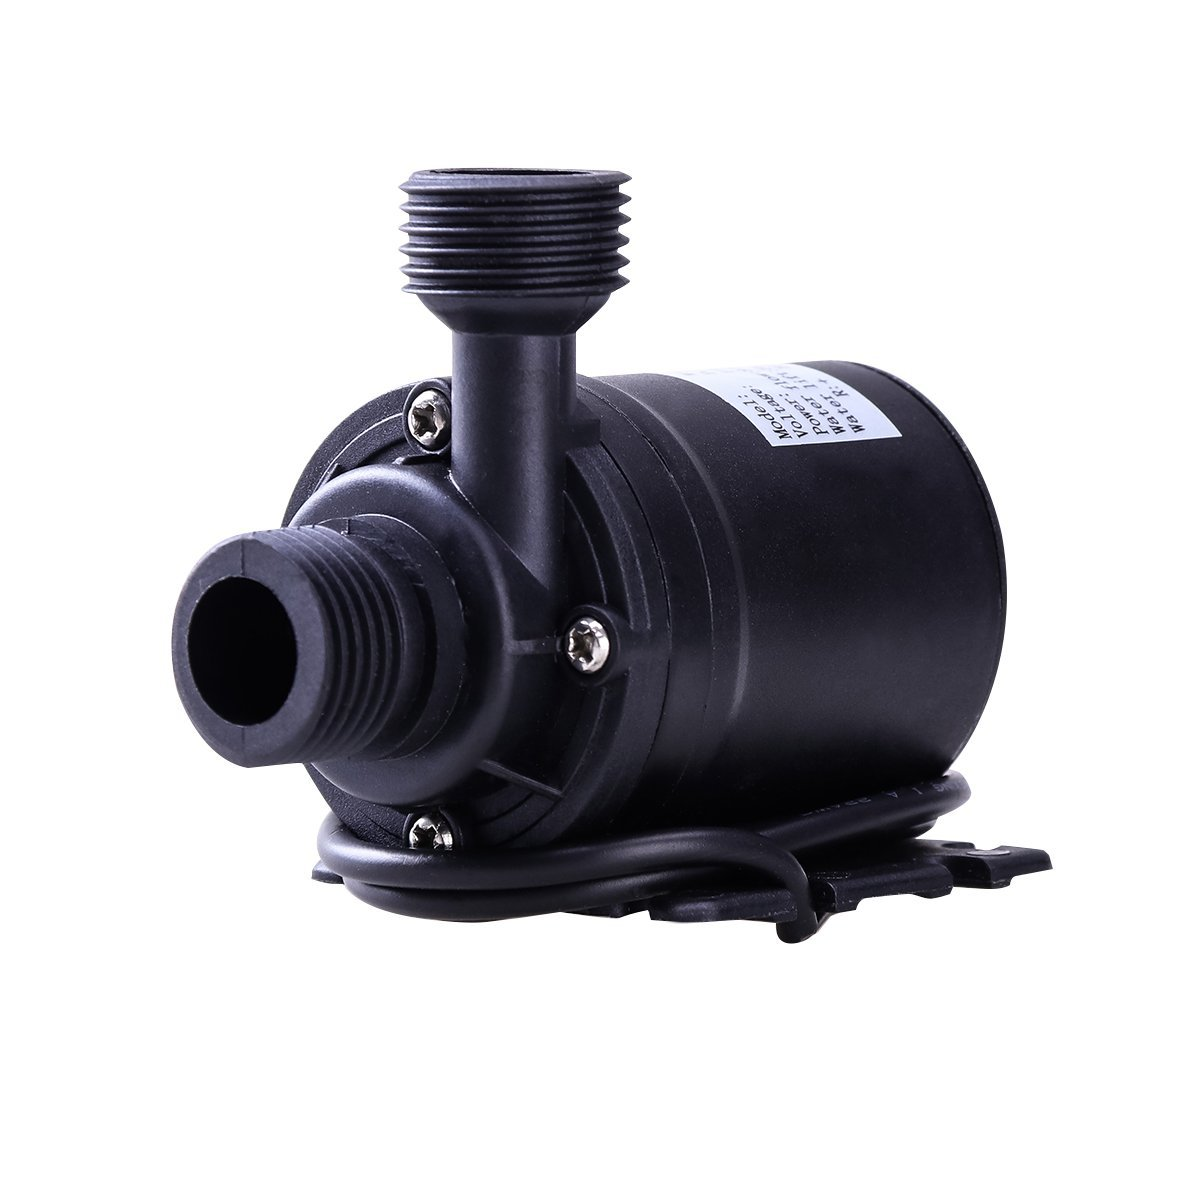
\includegraphics[width=0.5\textwidth]{images/pompe}
\end{figure}

Vous trouverez facilement ce genre de pompes sur amazon ou ebay en
y recherchant ''pompe 12V''. Il est cependant moins évident d'en
trouver avec des délais de livraison courts, mais ça se trouve. Les
principaux critères de choix pour la pompe sont :
\begin{itemize}
\item la tension de fonctionnement
\item la consommation électrique
\item la différence de pression que la pompe peut générer, elle est souvent
renseignée sous la forme d'un nombre de mètres (5M par exemple). Il
faut alors calculer à quoi ça correspond en pression hydrostatique.
Si vous voulez trouver des ordres de grandeur pour savoir de quelle
pression vous avez besoin, vous pouvez lire des articles sur le watercooling
de PC, qui se rapproche pas mal de notre problème. Sinon, une valeur
de 3 à 5 mètres devrait par expérience être largement suffisante.
\item le débit
\item les dimensions et la masse (ce serait con de prendre une pompe surdimensionnée)
\item la résistance à l'eau salée si besoin (si ce n'est pas mentionné,
pensez à rincer la pompe à l'eau douce après chaque utilisation en
eau salée)
\item le type de connectique : vous remarquerez qu'on ne trouve pas de pompes
munies de connexions rapides. Il faudra donc munir votre pompe d'adaptateurs,
que nous verrons un peu plus loin. Ceci n'est possible qu'avec les
pompes munies de connecteurs à vis.
\end{itemize}

\section{Echangeur eau-air}

\begin{figure}[h]
\caption{Echangeur eau-air}

\centering{}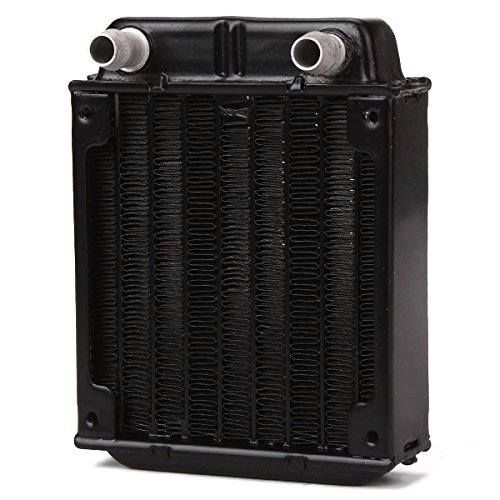
\includegraphics[width=0.5\textwidth]{images/radiateur}
\end{figure}

Ce type de produit peut servir à refroidir l'air à l'intérieur d'un
boîtier ou alors à dissiper la chaleur du circuit de refroidissement
à l'air extérieur. Il s'agit ici d'un ''refroidisseur ou radiateur
de watercooling'' (notez que ce modèle peut accueillir un ventilateur
de PC). Vous pouvez en trouver sur amazon et ebay (pensez à chercher
en anglais éventuellement) et une nouvelle fois, il s'agit d'arriver
à en trouver avec des délais d'expédition raisonnables. Les critères
de choix sont ici :
\begin{itemize}
\item les dimensions, que ce soit au niveau de l'encombrement ou de la surface
d'échange thermique.
\item le type de connectique : là encore, pas de connexions rapides, mais
pensez à prendre un modèle avec connecteurs à pas de vis, dans lesquels
on pourra visser des adaptateurs, que nous verrons plus loin.
\end{itemize}

\section{Adaptateurs raccord fileté - connexion rapide}

Si vous avez acheté des composants ne disposant pas de connexions
rapides, assurez vous qu'ils disposent de connecteurs filetés suivant
la norme BSP (British Standard Pipe). Le type de filetage peut malheureusement
être indiqué de plusieurs façons différentes. Par exemple, pour un
filetage d'un quart de pouce, on peut trouver ''BSP 1/4'' ou ''G
1/4'' (le G veut dire gaz, le filetage gaz étant un synonyme de BSP).
Si vous tombez sur les appelations BSPP et BSPT, il s'agit de deux
variantes du BSP. Pour plus d'informations sur toutes ces appelations,
ainsi qu'une liste des différentes dimensions de filetage existantes,
rendez vous sur la page wikipedia intitulée ''Filetage gaz''.

Une fois que vous avez déterminé le type de connecteur (BSP, male
ou femelle, d'un certain diamètre), vous pourrez trouver le bon adaptateur
dans la catégorie ''Metric Pneumatic Push Fit Compressed Air Fittings''
sur le site d'AFS. 

\begin{figure}[h]
\caption{Adaptateur BSP 1/4 femelle vers 8mm push fit}

\centering{}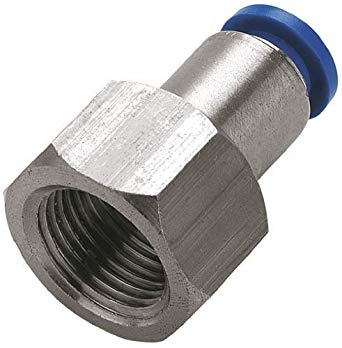
\includegraphics[width=0.4\textwidth]{images/threaded_adaptor.jpg}
\end{figure}

Vous pourrez ensuite visser les adaptateurs sur votre composant pour
le munir de connexions rapides. Attention cependant à assurer l'étanchéité
de ce raccordement par vissage. Il faut pour cela enduire le pas de
vis avant de visser. La meilleure façon de le faire est d'utiliser
du ''PTFE tape'' (vous pouvez trouver des vidéos sur youtube sur
son utilisation, et vous en procurer sur amazon).

\section{Réservoir d'eau}

Une façon simple de réaliser un réservoir d'eau est d'utiliser un
petit boîtier étanche (d'indice de protection élevé) muni de bulkheads
pour l'entrée et la sortie d'eau.

\section{Mise en place d'un circuit de refroidissement élaboré}
Le variateur utilisé pour contrôler et alimenter le moteur a besoin d'eau pour se refroidir. Il a donc fallut mettre en place un circuit de refroidissement.
Lors de l'édition 2018 de l'Hydrocontest, les équipes se sont rendues compte que la batterie avait une température à partir de laquelle la tension chutait jusqu'à atteindre 0V. Il est donc aussi nécessaire de refroidir la batterie.

Il a donc été décidé d'opter pour un circuit de refroidissement composé de 2 sous-circuit:
\begin{description}
\item[Circuit eau douce:]C'est ce circuit qui serait en contact avec le variateur et la batterie.
\item[Circuit eau de mer:]C'est le circuit qui "apporterait le froid".
\end{description}


Un circuit de refroidissement en 2 parties a été décidé afin de d'avoir une plus grande robustesse. En effet, on aurait alors le circuit en contact avec les éléments électriques auquel on ne toucherait presque jamais. De plus, nous allons avoir besoin de faire une plaque en cuivre pour refroidir la batterie et l'eau de mer réagit mal avec le cuivre.

\chapter{Passage de cables étanche entre un boîtier et l'extérieur}

\begin{figure}[h]
\caption{Presse étoupe}

\centering{}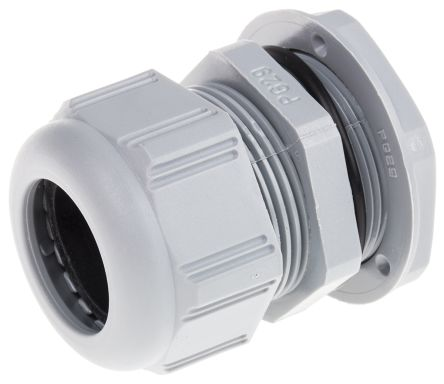
\includegraphics[width=0.5\textwidth]{images/presse_etoupe.jpg}
\end{figure}

Le produit idéal pour ce besoin est le presse-étoupe (cable gland
en anglais). N'hésitez pas à rechercher ce mot sur youtube afin de
voir comment ça marche. Vous en trouverez en grande quantité et à
très bon prix chez le fournisseur tme.eu. Le principal critère de
choix est le diamètre maximal de cable (et de connecteur) que vous
arriverez à faire passer à l'intérieur. Si vous devez faire passer
un connecteur à travers un presse-étoupe, faites attention à ses dimensions
!

\chapter{Bilan : fournisseurs évoqués}

J'ai déjà présenté les fournisseurs que j'ai utilisés pour les différents
produits évoqués, mais il est intéressant d'en faire un bilan, afin
d'avoir une vision globale des différentes possibilités pour se fournir
en différents types de matériel.
\begin{description}
\item[ebay :] vendeur electron-discount : petits composants électroniques,
expédition rapide de France
\item[tme.eu :] gros fournisseur à la manière de RS, mais avec un meilleur
choix et des meilleurs prix pour tout ce qui concerne l'implantation
de l'électronique (boîtiers, connexions étanches, antennes, cables
pour antennes, interrupteurs d'urgence...etc). Livraison très rapide
comme souvent avec ces fournisseurs, bien que les entrepôts soient
en Pologne
\item[rs components :] le gros fournisseur de référence, qui a la particularité
de proposer quelques produits utiles pour le circuit de refroidissement
(notamment les connexions push fit)
\item[advanced fluid solutions (afs) :] choix incomparable pour réaliser
des circuits hydrauliques ou pneumatiques, expédition du Royaume Uni
plutôt rapide (une semaine en gros)
\item[hobbyking, banggood :] choix énorme et meilleurs prix pour tout le
matériel utilisé en modélisme, attention cependant aux délais d'expédition
puisque leurs entrepôts principaux sont en Chine (sélectionner les
entrepôts européens sur hobbyking)
\item[amazon :] très bien pour les produits suffisament courants pour être
dans les entrepôts d'amazon (fusibles, wagos, connecteurs JST, PTFE
tape...etc), qu'il est souvent possible d'acheter sous forme d'assortiments
ou de kits
\item[robotshop :] il est rare que les produits qu'on y trouve ne soient
pas présents chez un autre des fournisseurs mentionnés ci-dessus,
cependant ce site est parfaitement adapté pour un projet de mécatronique,
car il s'adresse aux gens menant des projets proches de la robotique
/ de l'électronique sans être des professionnels. C'est sûrement le
site qui couvre la plus grande part de vos besoins. De plus, ils ont
un entrepôt en France et la livraison est très rapide
\item[gotronic, france robotique :] similaires à robotshop, c'est toujours
bien d'avoir des alternatives
\item[kubii :] le meilleur site français pour se fournir en raspberry pi
\end{description}

Bien sûr, n'hésitez pas à chercher d'autres fournisseurs et à enrichir
cette liste. Comme vous l'aurez sans doute compris en lisant ce document,
faites preuve de persévérance quand vous cherchez des composants,
et n'hésitez pas à chercher en français et en anglais. 

Bon courage dans vos achats, et n'hésitez pas à me contacter si vous
avez des questions !


\part{Les partenaires}

\section{Mines}

\subsection{La DE}
Adresses en: prénom.nom@mines-paristech.fr

\begin{description}
\item[Yvon Gaignebet:]notre tuteur d’AE, responsable du cours de mécatronique.
\item[Emmanuel Ledoux:]responsable du cours d’AE avec Pierre Chauvet.
\item[Jacky Lech:]votre aide pour la partie construction et menuiserie
\item[Mathieu Mazière:]pas besoin de le présenter. Il est très intéressé par le projet.
\item[Zaza:]Qui ne connaît pas Zaza?
\item[Elie Hachem:]le tuteur des 2 premières équipes, et potentiellement une aide pour les parties CAO et CFD. 
\item[Pietro Tomé:]l’encadrant des BTS électronique.
\item[Frédéric Xerri:]l’encadrant des BTS mécanique.
\item[Michelle Efther:] elle est très intéressée par le projet, ça vaut le coup de la maintenir au courant
\item[Franck Spalony:]il travaillera avec vous dans le cadre de la mécatronique, c’est un des encadrants en charge de la partie CAO et 3Dexperience, il s’intéresse beaucoup au projet.
\item[Sabine Cantournet:]grâce à elle nous avons été interviewés par le photographe responsable de la communication aux Mines et nous avons fait la Une de leur site Internet.

\end{description}

\subsection{Les Alumnis}
\begin{itemize}
\item[Laurent Debenedetti:](ancien délégué général des Alumni) : laurent.debenedetti@gmail.com
\item[Sophie Philippe:](une des deux secrétaires des anciens, celle qui publie les articles dans la revue) : sophie.philippe@mines-paris.org
\end{itemize}

\section{Entreprises}

\subsection{Numeca}
C'est une entreprise qui produit un logiciel de CFD, FineMarine dont nous nous servons. Ils nous ont offert un séminaire à Bruxelle pour apprendre à utiliser le logiciel. C'est Léo Chabert qui y est allé.

Ils sont intéressés par les résultats que nous allons obtenir avec nos simulations (ils nous ont demandés des captures d'écrans de CFD mais nous n'avions pas encore utilisé FineMarine).
\begin{description}
\item[Steve Laldjee:]le responsable du partenariat avec Numeca : steve.laldjee@numeca.be
\end{description}


\subsection{Chomarat}
C'est l'entreprise qui nous a fournis gratuitement des échantillons de fibre de carbone.
\begin{description}
\item[Vicky Singery:]ingénieure de Chomarat, qui a pu nous envoyer gratuitement des tissus carbone pour réaliser le bateau) : vicky.singery@chomarat.com
\end{description}

\subsection{Le Chantier Naval de Bordeaux}
C'est Arthur Fourny qui a réussi à les démarcher à travers son stage ouvrier qu'il a effectué chez eux. D'ailleurs, il est toujours possible de faire un stage ouvrier à CNB pour apprendre les bases de la stratification.

En dehors des newsletter générales et informatives, toutes les personnes de CNB sont à contacter en rappelant le nom d’Arthur Fourny si vous avez besoin d’elles directement, tant que vous n’êtes pas connus auprès d’eux.
\begin{description}
\item[Alexandre Dauberville:]la personne que vous allez devoir rapidement contacter, c’est le responsable communication et marketing de CNB, c’est le responsable du partenariat, c’est lui qui pourra vous donner des sous et gérer la communication avec vous : a.dauberville@cnb.fr
\item[Cyril Boyer:] personne importante, à ne pas contacter directement sans prévenir le chef de projet. Un des dirigeants de CNB : c.boyer@cnb.fr
\item[Sandra Claeys:]personne importante, à ne pas contacter directement sans prévenir le trésorier et le chef de projet, trésorière de CNB : s.claeys@cnb.fr
\item[Frédéric Chevrier:]ingénieur au BE, à contacter pour les questions concernant la plomberie ou le moteur : f.chevrier@cnb.fr
\item[Lionel Descatmat:]technicien composite, à contacter pour des questions pratiques concernant le matériel, l’utilisation des produits … : l.descatmat@cnb.fr
\item[Vincent Karsenty]expert en moule/moulage à CNB, très gentil, à contacter pour son expertise sur les questions de travail du composite et de moule : v.karsenty@cnb.fr
\item[Ivan Baler:]ingénieur du bureau d’étude, spécialiste des questions de résistance des matériaux, des structures et des formes de bateau : i.baler@cnb.fr
\item[Etienne Fleurant:]ingénieur du bureau d’étude, lui aussi spécialiste des questions de résistance des matériaux, des structures et des formes de bateau, à contacter en priorité car plus impliqué dans le projet : e.fleurant@cnb.fr
\end{description}

\subsection{Schlumberger}
C'est Alexandre Levesque qui a réussi à les démarcher à travers son stage de césure. 

Ils sont plutôt investi dans le projet et intéressé dans l'utilisation que nous allons faire des capteurs qu'ils ont sponsorisés (LIDAR, IMU et station GPS RTK).

\begin{description}
\item[Stephane Vannuffelen:]un des contacts d’Alexndre Levesque chez Schlum : svannuffelen@slb.com
\item[A Croux:]un des contacts d’Alexndre Levesque chez Schlum : acroux@slb.com

\end{description}

\subsection{Missler Software}
C'est l'un de nos sponsors que nous avons eu grâce au père de Jean-Baptiste Arber qui est l'un des dirigeants de Missler Software, entreprise de logiciels dont le produit phare est Topsolid, un logiciel de CAO. 

Il est très important de les nommer TopSolid dans toute la communication faite.

\subsection{Cirtes}
C'est l'entreprise qui a fournis le moule en mousse PU pour le bateau léger.

\begin{description}
\item[Hugo Ricatte:]un technicien haut placé avec qui nous avons discuté de toutes les questions techniques liées à la fabrication et à l’utilisation du moule
 : hugo.ricatte@cirtes.fr
\item[David Di Giuseppe:]une personne plus haut placée que Hugo et qui gère plutôt la partie achat, partenariat, réductions … : david.digiuseppe@cirtes.fr
\end{description}

\subsection{Autres}

\begin{description}
\item[Marc Pommelet:]pdg de Sistre, une boîte qui nous a fourni le logiciel Maat Hydro, dont nous ne nous sommes jamais servi : sistre@otenet.gr
\item[Jean Christophe Guillaumin:]le pdg de Multicoques Mag, magazine dans lequel vous avez tout intérêt de continuer à publier ! C’est également le papa de Jean Baptiste Guillaumin, un Mineur que vous allez rencontrer après son retour de césure : jcg@multihulls-world.com
\item Un contact chez Voiles et Voiliers (à tenter de contacter pour publier chez lui) : L.MADELINE@voilesetvoiliers.com
\item Sébastien - sebastien@gseadesign.com , Benjamin - benjamin@gseadesign.com , Damien - damiend@gseadesign.com  (trois employés de Gsea Design, pouvant peut-être vous filer un coup de main pour le design des foils ou de la CAO)
\end{description}

\section{Particuliers}
-	Fourny 
o	Carine et Alexandre Fourny (les parents d’Arthur) : acac.fourny@wanadoo.fr
o	Alain Fourny, (grand père d’Arthur) :  fournyalain@orange.fr
-	Famille Levesque :  fb.levesque@wanadoo.fr
-	Famille Goutaland :  l.goutaland@boissonstores.fr
-	René Lempereur (passionné d’aéromodélisme, de construction de modèles réduits d’avion … voir son site internet pour plus d’informations) : a-s-a@wanadoo.fr
-	Arnaud Mistre (celui qui nous a fait la CAO de Billy l’ancien, copain d’Elie, très intéressé par le projet) : arnaud@mistre.fr


\part{Les équipes hydromines}
Vous trouverez dans cette partie les membres des équipes des différentes années ainsi que leurs contacts afin que vous puissiez les joindre en cas de question ou en cas de problèmes. Il ne faut pas hésiter à leur demander conseils ou explications sur ce qui a été fait les années précédentes, ils seront ravis de vous aider.

\section{2016-2018}

\begin{description}
\item[Alexandre Levesque:]Chef de projet
\item[Antonin Succo:]Responsable mécanique et logistique
\item[Arthur Fournier:]Trésorier et responsable des relations avec les partenaires
\item[Bandouin Lecerf:]
\item[Ulysse Réglade:] Responsable électronique
\item[Jean-Baptiste Arber:] Responsable électronique
\end{description}

\section{2017-2019}

\begin{description}
\item[Victor Amblard:] Chef de projet
\item[Lauriwen Risset:] Responsable communication
\item[Léo Chabert:] Responsable logistique
\item[Thomas Gossard:]Trésorier et responsable électronique
\item[Camille Gaie-Bellile:] Aide. Elle a réalisé son stage au Chantier Naval de Bordeaux. Cela lui a permis d'apprendre à stratifier.
\end{description}

\section{2018-2020}

\end{document}